% Created 2024-04-13 Sat 11:30
% Intended LaTeX compiler: pdflatex
\documentclass[11pt]{article}
\usepackage[utf8]{inputenc}
\usepackage[T1]{fontenc}
\usepackage{graphicx}
\usepackage{longtable}
\usepackage{wrapfig}
\usepackage{rotating}
\usepackage[normalem]{ulem}
\usepackage{amsmath}
\usepackage{amssymb}
\usepackage{capt-of}
\usepackage{hyperref}
\usepackage{siunitx}
\author{Hankertrix}
\date{\today}
\title{Mechanics Of Materials Cheat Sheet}
\hypersetup{
 pdfauthor={Hankertrix},
 pdftitle={Mechanics Of Materials Cheat Sheet},
 pdfkeywords={},
 pdfsubject={},
 pdfcreator={Emacs 29.3 (Org mode 9.6.15)}, 
 pdflang={English}}
\begin{document}

\maketitle
\setcounter{tocdepth}{2}
\tableofcontents \clearpage
\section{Definitions}
\label{sec:orgfe71d07}

\subsection{Member}
\label{sec:orgb1db66b}
An object that experiences stress. It can be something like a rod.

\subsection{Two-force member}
\label{sec:org925641d}
A two-force member just means that there is no transverse load between the pinned ends of an object.

\subsection{Axial loading}
\label{sec:org6d61e6d}
Axial loading just means that the object is loaded on a plane parallel to the object's axis. For example, a beam is axially loaded when the forces are on the ends of the beam.

\subsection{Normal stress (\(\sigma\))}
\label{sec:org5ac0d9a}
The force intensity on a section of an object due to axial loading is called normal stress. It is called normal because the force is perpendicular to the plane of the exposed section where the object is cut.

\subsection{Centroid}
\label{sec:org199ac79}
The centroid is the centre of the object.

\subsection{Centric (concentric) loading}
\label{sec:org6c80214}
\begin{itemize}
\item A uniform distribution of stress in a section infers that the line of action for the result of the internal forces passes through the \textbf{centroid} of the section.
\item A uniform distribution of stress is only possible if the concentrated loads on the end sections of two-force members are applied at the centre of the sections at the ends of the object.
\end{itemize}

\newpage

\subsection{Eccentric loading}
\label{sec:org9307769}
\begin{itemize}
\item Axial loading which does not pass through the centroid of a section produces internal forces equivalent to an axial force and a bending moment.
\item If a two-force member is eccentrically loaded, then the resultant of the stress distribution in a section must yield an axial force and a moment.
\item The stress distributions in eccentrically loaded members cannot be uniform or symmetric.
\item The direction of the force and the resultant moment can be found through equilibrium.
\end{itemize}

\subsection{Shearing stress (\(\tau\))}
\label{sec:org2c26c8b}
\begin{itemize}
\item Two forces are applied transversely to an object results in a shearing force
\item The resultant of the internal shear force distribution is known as the shear of the section and is equal to the load.
\end{itemize}

\[\tau_{avg} = \frac{F}{A}\]

Where:
\begin{itemize}
\item \(\tau_{avg}\) is the average shearing stress
\item \(F\) is the shear force
\item \(A\) is the cross-sectional area of the shearing surface, which is the area of the surface that is being sheared.
\end{itemize}

For a \textbf{single shear}, the formula for shearing stress is the above. However, for \textbf{double} shear, the force needs to be divided by 2.

\newpage

\subsection{Bearing stress (\(\sigma_b\))}
\label{sec:org2325a1b}
\begin{itemize}
\item Bolts, rivets, and pins create stresses on the points of contact of the objects.
\item The average force intensity is called bearing stress.
\end{itemize}

\[\sigma_b = \frac{F}{A} = \frac{F}{t \, d}\]

Where:
\begin{itemize}
\item \(\sigma_b\) is the bearing stress
\item \(F\) is the force applied by the pin
\item \(A\) is the projected area
\item \(t\) is the thickness of the material the pin is in contact with
\item \(d\) is the diameter of the pin
\end{itemize}

\newpage

\subsection{Factor of safety (\(FS\))}
\label{sec:orgd72a6c8}
Factor of safety considerations:
\begin{itemize}
\item Uncertainty in material properties
\item Uncertainty of loadings
\item Uncertainty of analyses
\item Number of loading cycles
\item Types of failure
\item Maintenance requirements and deterioration effects
\item Importance of member to structure integrity
\item Risk to life and property
\item Influence on machine function
\end{itemize}

\[FS = \frac{\sigma_u}{\sigma_{all}}\]

Where:
\begin{itemize}
\item \(FS\) is the factor of safety
\item \(\sigma_u\) is the ultimate stress
\item \(\sigma_all\) is the allowable stress
\end{itemize}

\subsection{Normal strain (\(\varepsilon\))}
\label{sec:orgba04cbd}
\[\varepsilon = \frac{\delta}{L}\]

Where:
\begin{itemize}
\item \(\varepsilon\) is the normal strain
\item \(\delta\) is the extension of the object under strain
\item \(L\) is the length of the object
\end{itemize}

\subsection{Elastic behaviour}
\label{sec:org154da79}
Elastic behaviour is when the strain disappears when the stress is removed. The largest stress for which this occurs is called the elastic limit.

\subsection{Plastic (inelastic) behaviour}
\label{sec:org7e96961}
Plastic behaviour is when the strain does not return to zero after the stress is removed.

\subsection{Hooke's Law: Modulus of Elasticity (Stiffness) (\(E\))}
\label{sec:orgb157683}
For uniaxial stress:
\[\sigma = E \varepsilon \qquad E = \frac{\sigma}{\varepsilon}\]

Where:
\begin{itemize}
\item \(\sigma\) is the normal stress
\item \(\varepsilon\) is the normal strain
\item \(E\) is Young's Modulus or Modulus of Elasticity or Elastic Modulus
\end{itemize}

The strength of a material is affected by alloying, heat treating, and manufacturing process but the stiffness of a material (Modulus of Elasticity) is not.

\subsection{Fatigue}
\label{sec:orgbbed717}
\begin{itemize}
\item Fatigue properties are shown on stress vs number of cycles to failure graphs.
\item A member may fail due to fatigue at stress levels significantly below the ultimate strength if subjected to many loading cycles.
\item When the stress is reduced below the \textbf{endurance limit}, fatigue failures do not occur for any number of cycles.
\end{itemize}

\newpage

\subsection{Poisson's ratio (\(\nu\))}
\label{sec:orgc4aef2f}
\begin{itemize}
\item For a slender bar subjected to axial loading:
\[\varepsilon_x = \frac{\sigma_x}{E} \qquad \sigma_y = \sigma_z = 0\]

\item The elongation in the \(x\)-direction is accompanied by a contraction in the other directions. Assuming that the material is isotropic (no directional dependence),
\[\varepsilon_y = \varepsilon_z \ne 0\]
\end{itemize}

Poisson's ratio is defined as:
\[\nu = \left| \frac{\text{lateral strain}}{\text{axial strain}} \right| = - \frac{\varepsilon_y}{\varepsilon_x} = - \frac{\varepsilon_z}{\varepsilon_x}\]

Where:
\begin{itemize}
\item \(\nu\) is the Poisson's ratio
\item \(\varepsilon_x\) is the normal strain on the object in the \(x\)-direction
\item \(\varepsilon_y\) is the normal strain on the object in the \(y\)-direction
\item \(\varepsilon_z\) is the normal strain on the object in the \(z\)-direction
\end{itemize}

\subsection{Generalised Hooke's Law}
\label{sec:orgbf3a5a2}
\[\varepsilon_x = + \frac{\sigma_x}{E} - \frac{\nu \sigma_y}{E} - \frac{\nu \sigma_z}{E}\]
\[\varepsilon_y = + \frac{\sigma_y}{E} - \frac{\nu \sigma_x}{E} - \frac{\nu \sigma_z}{E}\]
\[\varepsilon_z = + \frac{\sigma_z}{E} - \frac{\nu \sigma_x}{E} - \frac{\nu \sigma_y}{E}\]

Where:
\begin{itemize}
\item \(\varepsilon\) is the normal strain on the object in the respective \(x\), \(y\) and \(z\) directions.
\item \(\nu\) is the Poisson's ratio
\item \(E\) is the elastic modulus
\end{itemize}

\subsection{Shearing strain (\(\gamma\))}
\label{sec:orgf3e8c24}
\begin{itemize}
\item A cubic element subjected to a shearing stress will deform into a rhomboid. The corresponding \textbf{shear strain} is quantified in terms of the change in angle between the sides.
\item Shearing stress in one plane only affects shearing strain in the same plane.
\item For small strains, \(\tan \gamma \approx \gamma\):
\[\tau_{xy} = G \gamma_{xy}\]
\[\tau_{yz} = G \gamma_{yz}\]
\[\tau_{zx} = G \gamma_{zx}\]

Where:
\begin{itemize}
\item \(\tau\) is the shearing stress in the respective planes
\item \(G\) is the shear modulus
\item \(\gamma\) is the \textbf{shearing strain}, or the change in angle \textbf{in radians} due to shearing in the respective planes
\end{itemize}
\end{itemize}

\subsection{Modulus of rigidity (Shear modulus) (\(G\))}
\label{sec:org1e98521}
\[G = \frac{\tau}{\gamma}\]

Where:
\begin{itemize}
\item \(G\) is the modulus of rigidity or the shear modulus
\item \(\tau\) is the shearing stress
\item \(\gamma\) is the \textbf{shearing strain}, or the change in angle \textbf{in radians} due to shearing
\end{itemize}

\[G = \frac{E}{2(1 + \nu)}\]

Where:
\begin{itemize}
\item \(G\) is the shear modulus
\item \(E\) is the elastic modulus
\item \(\nu\) is Poisson's ratio
\end{itemize}

\subsection{Net torque due to internal stresses (\(T\))}
\label{sec:org6b96c68}
The net internal shearing stress is an internal torque that is \textbf{equal and opposite to the applied torque}.

\[T = \int \rho \, dF = \int \rho (\tau dA)\]

Where:
\begin{itemize}
\item \(T\) is the internal torque
\item \(\rho\) is the radius at any point
\item \(dF\) is the force on an infinitesimal element of the cross-sectional area
\item \(\tau\) is the internal shearing stress on the object
\item \(dA\) is an infinitesimal element of the cross-sectional area
\end{itemize}

Unlike the normal stress due to axial loads, the distribution of shearing stresses due to torsional loads \textbf{cannot be assumed uniform}.

\newpage

\subsection{Shearing strain due to torsion (\(\gamma\))}
\label{sec:org02c11be}
\[L \gamma = \rho \phi \text{ or } \gamma = \frac{\rho \phi}{L}\]

Where:
\begin{itemize}
\item \(L\) is the length of the shaft
\item \(\gamma\) is the \textbf{shearing strain}, or the change in angle \textbf{in radians} due to shearing
\item \(\rho\) is the radius at any point
\item \(\phi\) is the twisting angle
\end{itemize}

Shearing strain is proportional to the twisting angle and the radius of the shaft.
\\[0pt]

As \(\rho \rightarrow c\),
\[\gamma_{max} = \frac{c \phi}{L}\]
\[\gamma = \frac{\rho}{c} \gamma_{max}\]

Where:
\begin{itemize}
\item \(\gamma_{max}\) is the \textbf{maximum shearing strain}, or the maximum change in angle \textbf{in radians} due to shearing
\item \(c\) is the outer radius of the shaft
\item \(L\) is the length of the shaft
\item \(\gamma\) is the \textbf{shearing strain}, or the change in angle \textbf{in radians} due to shearing
\item \(\rho\) is the radius at any point
\item \(\phi\) is the twisting angle
\end{itemize}

\subsubsection{Shearing stress in elastic range (\(\tau\))}
\label{sec:org94b69ac}
Multiplying the previous equation by the shear modulus:
\[G \gamma = \frac{\rho}{c} G \gamma_{max}\]

Where:
\begin{itemize}
\item \(G\) is the shear modulus
\item \(\gamma\) is the \textbf{shearing strain}, or the change in angle \textbf{in radians} due to shearing
\item \(\rho\) is the radius at any point
\item \(c\) is the outer radius of the shaft
\end{itemize}

From Hooke's law, \(\tau = G \gamma\):
\[\tau = \frac{\rho}{c} \tau_{max}\]

Where:
\begin{itemize}
\item \(\tau\) is the shearing stress due to torsion
\item \(\rho\) is the radius at any point
\item \(c\) is the outer radius of the shaft
\item \(\tau_{max}\) is the maximum shearing stress due to torsion
\end{itemize}

The shearing stress due to torsion varies \textbf{linearly} with the \textbf{radial position} in the section.

\subsection{Polar moment of inertia (\(J\))}
\label{sec:org2f9b797}

\subsubsection{Solid circular shaft}
\label{sec:orgecc9bce}
\[J = \frac{1}{2}\pi c^4 = \frac{1}{32}\pi d^4\]

Where:
\begin{itemize}
\item \(J\) is the polar moment of inertia
\item \(c\) is the outer radius of the shaft
\item \(d\) is the diameter of the shaft
\end{itemize}

\subsubsection{Hollow circular shaft}
\label{sec:org85d4e38}
\[J = \frac{1}{2} \pi \left(r_2^4 - r_1^4 \right) = \frac{1}{32} \pi \left(d_2^4 - d_1^4 \right)\]

Where:
\begin{itemize}
\item \(J\) is the polar moment of inertia
\item \(r_2\) is the \textbf{external} radius
\item \(r_1\) is the \textbf{internal} radius
\item \(d_2\) is the \textbf{external} diameter
\item \(d_1\) is the \textbf{internal} diameter
\end{itemize}

\subsection{Elastic torsion formula}
\label{sec:org9ffdaeb}
\[\tau_{max} = \frac{Tc}{J}\]
\[\tau = \frac{T \rho}{J}\]

Where:
\begin{itemize}
\item \(\tau_{max}\) is the maximum shearing stress on the shaft
\item \(T\) is the torque on the shaft
\item \(c\) is the outer radius of the shaft
\item \(J\) is the polar moment of inertia
\item \(\tau\) is the shearing stress on the shaft
\item \(\rho\) is the radius at any point on the shaft
\end{itemize}

\newpage

\subsection{Angle of twist in elastic range (\(\phi\))}
\label{sec:org0e62945}
\[\phi = \frac{TL}{GJ}\]

Where:
\begin{itemize}
\item \(\phi\) is the twisting angle
\item \(T\) is the torque on the shaft
\item \(L\) is the length of the shaft
\item \(G\) is the shear modulus
\item \(J\) is the polar moment of inertia
\end{itemize}

If the torsional loading or shaft cross-section changes along the length, the angle of rotation is found as the sum of segment rotations.
\[\phi = \sum_i \frac{T_i L_i}{G_i J_i}\]

Where:
\begin{itemize}
\item \(\phi\) is the twisting angle
\item \(T_i\) is the torque on the respective part of the shaft
\item \(L_i\) is the length of the respective part of the shaft
\item \(G_i\) is the shear modulus for the respective part of the shaft
\item \(J_i\) is the polar moment of inertia for the respective part of the shaft
\end{itemize}

\subsection{Power due to torque (\(P\))}
\label{sec:org2d8b64e}
\[P = T \omega = 2 \pi f T\]

Where:
\begin{itemize}
\item \(P\) is the power due to the applied torque
\item \(T\) is the torque applied
\item \(\omega\) is the angular velocity
\item \(f\) is the frequency
\item \(t\) is the period
\end{itemize}

\subsubsection{Torque in terms of power (\(T\))}
\label{sec:orgdd0405f}
\[T = \frac{P}{\omega} = \frac{P}{2 \pi f}\]

Where:
\begin{itemize}
\item \(P\) is the power due to the applied torque
\item \(T\) is the torque applied
\item \(\omega\) is the angular velocity
\item \(f\) is the frequency
\item \(t\) is the period
\end{itemize}

\subsection{Bending moment (\(M\))}
\label{sec:org7ca223a}
Bending moment is the reaction induced in a structural element when an external force or moment is applied to the element, causing the element to bend.

\subsection{Pure bending}
\label{sec:orgd43de42}
Pure bending is a condition of stress where a bending moment is applied to a beam without the simultaneous presence of axial, shear or torsional forces. Basically, pure bending just means that the object \textbf{only} experiences bending.

\subsection{Transverse loading}
\label{sec:orgd38aeeb}
Concentrated or distributed transverse load produces internal forces equivalent to a shear force and a bending moment.

\subsection{Principle of superposition}
\label{sec:org579c0a5}
The normal stress due to pure bending may be combined with the normal stress due to axial loading, and the shearing stress due to shear loading, to find the complete state of stress.

\subsection{Neutral axis (NA)}
\label{sec:orge52ae33}
The neutral axis is the axis of the \textbf{bending moment}. The neutral axis passes through the centroid of the cross-section.

\subsection{Normal strain due to bending (\(\varepsilon_x\))}
\label{sec:org080737c}
\[\varepsilon_x = - \frac{y}{c} \left| \varepsilon_m \right|\]

Where:
\begin{itemize}
\item \(\varepsilon_x\) is the normal strain due to the bending moment
\item \(y\) is the distance from the neutral axis to the point of interest
\item \(c\) is the distance from the centroid of the object to the outer surface
\item \(\varepsilon_m\) is the maximum normal strain due to the bending moment
\end{itemize}

\subsubsection{Maximum normal strain (\(\varepsilon_m\))}
\label{sec:orgd788598}
\[\varepsilon_m = \frac{c}{\rho}\]
\[\rho = \frac{c}{\left| \varepsilon_m \right|}\]

Where:
\begin{itemize}
\item \(\varepsilon_m\) is the maximum normal strain due to the bending moment
\item \(c\) is the distance from the centroid of the object to the outer surface
\item \(\rho\) is the distance from the centroid to the centre of the circle
\end{itemize}

\newpage

\subsection{Normal stress due to bending (\(\sigma_x\))}
\label{sec:org10f6079}
\begin{itemize}
\item The stress due to bending is always uniaxial.
\item The stress due to bending must be parallel to the axis of the object, which is in the x-direction.
\end{itemize}

For a linearly elastic material:
\[\sigma_x = E \varepsilon_x = - \frac{y}{c} E \varepsilon_m\]
\[\sigma_x = - \frac{y}{c} \sigma_m\]
\[\sigma_x = \frac{My}{I}\]

Where:
\begin{itemize}
\item \(\sigma_x\) is the normal stress due to the bending moment
\item \(E\) is the elastic modulus
\item \(\varepsilon_x\) is the normal strain due to the bending moment
\item \(y\) is the distance from the neutral axis to the point of interest
\item \(c\) is the distance from the centroid of the object to the outer surface
\item \(M\) is the total bending moment
\item \(\varepsilon_m\) is the maximum normal strain due to the bending moment
\item \(\sigma_m\) is the maximum normal stress due to the bending moment
\end{itemize}

\newpage

\subsubsection{Maximum normal stress (\(\sigma_m\))}
\label{sec:org358dc91}
\[\sigma_m = \left| \frac{Mc}{I} \right| = \left| \frac{M}{S} \right|\]

Where:
\begin{itemize}
\item \(\sigma_m\) is the maximum normal stress due to the bending moment
\item \(M\) is the total bending moment
\item \(c\) is the distance from the centroid of the object to the outer surface
\item \(I\) is the second moment of area
\item \(S\) is the section modulus, where \(S = \frac{I}{c}\)
\end{itemize}

\subsection{Second moment of area (\(I\))}
\label{sec:org109d100}
The second moment of area is \textbf{always perpendicular} to the shear force.

\subsubsection{Rectangular section}
\label{sec:org2aad64f}
\[I_{\text{NA}} = \frac{1}{12} bh^3\]

Where:
\begin{itemize}
\item \(I_{\text{NA}}\) is the second moment of area about the neutral axis
\item \(b\) is the base of the rectangular section
\item \(h\) is the height of the rectangular section
\end{itemize}

\subsubsection{Solid circular shaft}
\label{sec:orgb73d149}
\[I_{\text{NA}} = \frac{1}{4}\pi c^4 = \frac{1}{64}d^4 = \frac{J}{2}\]

Where:
\begin{itemize}
\item \(I_{\text{NA}}\) is the second moment of area about the neutral axis
\item \(c\) is the radius of the circular shaft
\item \(d\) is the diameter of the circular shaft
\item \(J\) is the polar moment of inertia
\end{itemize}

\subsubsection{Hollow circular shaft}
\label{sec:orgc9d0aee}
\[I_{\text{NA}} = \frac{1}{4}\pi \left(r_2^4 - r_1^4 \right) = \frac{1}{64}\pi \left(d_2^4 - d_1^4 \right) = \frac{J}{2}\]

Where:
\begin{itemize}
\item \(I_{\text{NA}}\) is the second moment of area about the neutral axis
\item \(r_2\) is the \textbf{external} radius
\item \(r_1\) is the \textbf{internal} radius
\item \(d_2\) is the \textbf{external} diameter
\item \(d_1\) is the \textbf{internal} diameter
\item \(J\) is the polar moment of inertia
\end{itemize}

\subsection{Section modulus (\(S\))}
\label{sec:org5ccbf4d}
\begin{itemize}
\item A beam with a larger section modulus will have a lower maximum stress.
\item A rectangular beam with greater depth will be more effective in resisting bending.
\item Structural steel beams are designed to have a large section modulus.
\end{itemize}

\[S = \frac{I_{\text{NA}}}{c}\]

Where:
\begin{itemize}
\item \(S\) is the section modulus
\item \(I_{\text{NA}}\) is the second moment of area about the neutral axis
\item \(c\) is the distance from the centroid of the object to the outer surface
\end{itemize}

\subsection{Parallel axis theorem}
\label{sec:org55aa444}
\[I = \sum \left(\bar{I} + Ad^2 \right) = \sum \left(\frac{1}{12} bh^3 + Ad^2 \right)\]

Where:
\begin{itemize}
\item \(I\) is the second moment of area of the object
\item \(\bar{I}\) is the second moment of area for an \textbf{individual} section of the object
\item \(A\) is the area of an \textbf{individual} section of the object
\item \(d\) is the distance from the centroid of the \textbf{individual} section from the centroid of the whole object
\item \(b\) is the base of an \textbf{individual} section of the object
\item \(h\) is the height of an \textbf{individual} section of the object
\end{itemize}

\subsection{Stress due to eccentric axial loading (\(\sigma\))}
\label{sec:org0cc8f3b}
Stress due to eccentric loading is found by superposing the uniform stress due to a concentric load and the linear stress distribution due to the bending moment.
\begin{align*}
\sigma &= \sigma_{\text{concentric}} + \sigma_{\text{bending}} \\
&= \frac{P}{A} \pm \frac{My}{I}
\end{align*}

\subsection{Concentrated loads}
\label{sec:orgfdd04c7}
Concentrated loads are basically point loads.

\subsection{Distributed loads}
\label{sec:orgb3b44b9}
Distributed loads are loads distributed over an area. Basically any load that isn't a point load or a concentrated load is a distributed load.

\subsection{Force}
\label{sec:org054c67b}
The word "force" just means a force-type quantity, which includes a concentrated force, moment or torque.

\subsection{Statically determinate beams}
\label{sec:org522fcad}
\begin{itemize}
\item Statically \textbf{determinate} beams are beams that have \textbf{only} the necessary amount of support.
\item Using the equilibrium equations for forces and moments is \textbf{sufficient} to find all the unknowns of a statically determinate beam.
\end{itemize}

\begin{center}
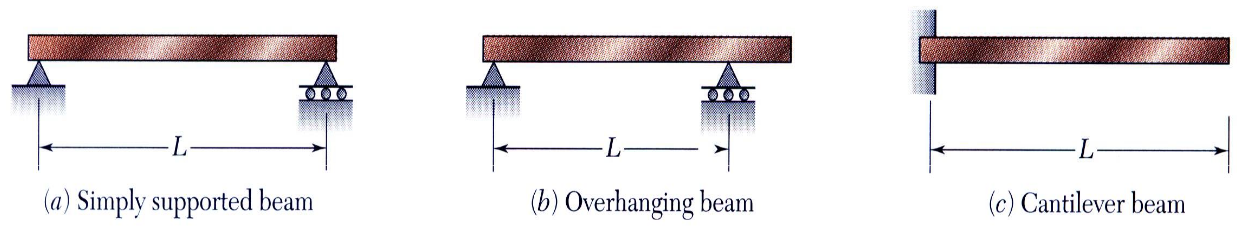
\includegraphics[width=.9\linewidth]{./images/statically-determinate-beams.png}
\end{center}

\subsection{Statically indeterminate beams}
\label{sec:org1c14a82}
\begin{itemize}
\item Statically \textbf{indeterminate} beam have \textbf{more} support than is strictly necessary.
\item Using the equilibrium equations for forces and moments is \textbf{insufficient} to find all the unknowns of a statically indeterminate beam.
\item Additional information is usually required to figure out all the unknowns of a statically indeterminate beam.
\end{itemize}

\begin{center}
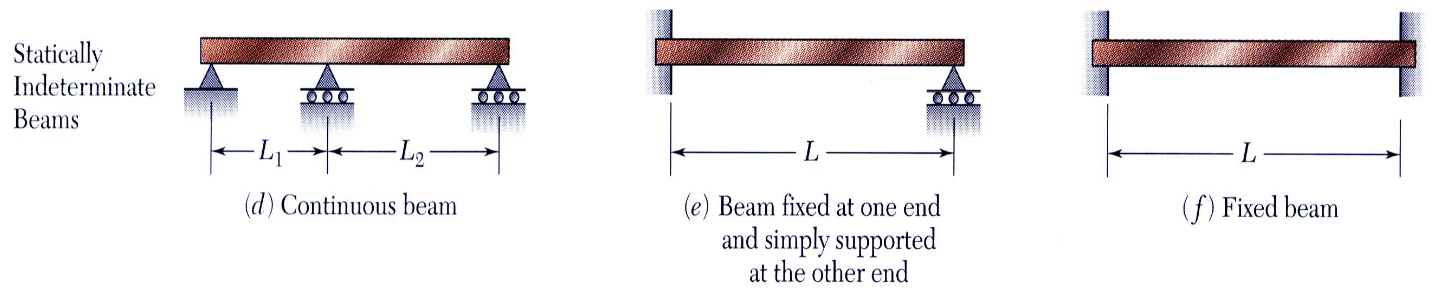
\includegraphics[width=.9\linewidth]{./images/statically-indeterminate-beams.png}
\end{center}

\newpage

\subsection{First moment of area about the neutral axis (\(Q\))}
\label{sec:org1170851}
\[Q = \int_{A} y \, dA = A \bar{y}\]

Where:
\begin{itemize}
\item \(Q\) is the first moment of area about the neutral axis
\item \(y\) is the distance from the neutral axis from a point on the object
\item \(dA\) is the infinitesimal area element
\item \(A\) is the area of the region of interest, which is the surface the force is acting on
\item \(\bar{y}\) is the distance from the neutral axis to the centroid of the area \(A\)
\end{itemize}

\subsubsection{For circular sections}
\label{sec:org2efd674}
Centroid of semicircular area is:
\[\bar{y} = \frac{4r}{3 \pi}\]

For a \textbf{solid} section:
\[Q = A \bar{y} = \frac{\pi r^2}{2} \frac{4r}{3 \pi} = \frac{2r^3}{3}\]

For a \textbf{hollow} section:
\[Q = \frac{2}{3} \left(r_2^3 - r_1^3 \right)\]

Where:
\begin{itemize}
\item \(Q\) is the first moment of area bout the neutral axis
\item \(\bar{y}\) is the distance from the neutral axis to the centroid of the area \(A\)
\item \(r\) is the radius of the semicircle
\item \(r_2\) is the outer radius of the semicircle
\item \(r_1\) is the inner radius of the semicircle
\end{itemize}

\subsection{Shear force due to bending}
\label{sec:org1f429c6}
\[F_{shear} = \frac{MQ}{I}\]

Where:
\begin{itemize}
\item \(F_{shear}\) is the shear force on the object. The direction of the force depends on whether the region is in compression or tension.
\item \(M\) is the total bending moment
\item \(Q\) is the first moment of area about the neutral axis
\item \(I\) is the second moment of area of the object
\end{itemize}

\subsection{Shear flow (force per unit length) (\(q\))}
\label{sec:org265429d}
\[q = \frac{dF}{dx} = \frac{dM}{dx} \frac{Q}{I} = \frac{VQ}{I}\]

Where:
\begin{itemize}
\item \(q\) is the shear flow
\item \(\frac{dF}{dx}\) is the shear force per unit length
\item \(\frac{dM}{dx}\) is the bending moment per unit length
\item \(Q\) is the first moment of the area of interest
\item \(I\) is the second moment of area of the entire section about the neutral axis
\item \(V\) is the total shear force at the section of interest
\end{itemize}

\newpage

\subsection{Shearing stress due to bending (\(\tau\))}
\label{sec:orgd6a1d8c}
\[\tau = \frac{q}{t} = \frac{VQ}{It} = \frac{VA \bar{y}}{It}\]

Where:
\begin{itemize}
\item \(\tau\) is the shearing stress due to bending
\item \(q\) is the shear flow, or the force per unit length
\item \(t\) is the width of the imaginary cut of interest. For hollow circular shafts, \(t\) is \textbf{twice the thickness of the shaft}, unless the \textbf{cut area} is only as thick as the \textbf{shaft thickness}, then it's just the \textbf{thickness of the shaft}.
\item \(V\) is the total shear force at the section of interest
\item \(Q\) is the first moment of the area of interest
\item \(I\) is the second moment of area of the entire section about the neutral axis
\item \(A\) is the area of interest
\item \(\bar{y}\) is the distance from the neutral axis to the centroid of the area \(A\)
\end{itemize}

\subsection{Plane stress}
\label{sec:org5119996}
Plane stress is a state of stress where 2 faces of a cubic element is free of stress. The state of stress is defined by:
\[\sigma_x, \sigma_y, \tau_{xy} \text{ and } \sigma_z = \tau_{zx} = \tau_{zy} = 0\]

\subsubsection{Examples}
\label{sec:orga4b1550}
\begin{itemize}
\item Thin plate subjected to forces acting in the mid-plane of the plate.
\item Any point on free surface not subjected to an external force.
\end{itemize}

\newpage

\subsection{Stress transformation equations}
\label{sec:orgcd33bd7}

\subsubsection{Sign conventions}
\label{sec:orgfa66116}
\begin{itemize}
\item The normal stress (\(\sigma\)) is \textbf{positive} if it is tensile.
\item The shearing stress (\(\tau\)) is \textbf{positive} if the line formed by the shearing stress has a \textbf{positive gradient}.
\item The rotation of the element (\(\theta\)) is positive when the element is rotated \textbf{anticlockwise} with respect to the \(x\)-axis.
\end{itemize}

\subsubsection{Normal stress (\(\sigma_{x'}\))}
\label{sec:org83977ad}
\[\sigma_{x'} = \frac{\sigma_x + \sigma_y}{2} + \frac{\sigma_x - \sigma_y}{2} \cos 2 \theta + \tau_{xy} \sin 2 \theta\]

Where:
\begin{itemize}
\item \(\sigma_{x'}\) is the normal stress of the element in the \(x\)-direction rotated \(\theta\) degrees \textbf{anticlockwise}.
\item \(\sigma_x\) is the normal stress of the element in the \(x\)-direction
\item \(\sigma_y\) is the normal stress of the element in the \(y\)-direction
\item \(\tau_{xy}\) is the shearing stress of the element in the \(xy\) plane.
\end{itemize}

Replacing \(\theta\) with \(\theta + 90\):
\[\sigma_{y'} = \frac{\sigma_x + \sigma_y}{2} + \frac{\sigma_x - \sigma_y}{2} \cos 2 \theta - \tau_{xy} \sin 2 \theta\]

Where:
\begin{itemize}
\item \(\sigma_{y'}\) is the normal stress of the element in the \(y\)-direction rotated \(\theta\) degrees \textbf{anticlockwise}.
\item \(\sigma_x\) is the normal stress of the element in the \(x\)-direction
\item \(\sigma_y\) is the normal stress of the element in the \(y\)-direction
\item \(\tau_{xy}\) is the shearing stress of the element in the \(xy\) plane.
\end{itemize}

\subsubsection{Shearing stress (\(\tau_{x'y'}\))}
\label{sec:org9201be9}
\[\tau_{x'y'} = - \frac{\sigma_x - \sigma_y}{2} \sin 2 \theta + \tau_{xy} \cos 2 \theta\]

Where:
\begin{itemize}
\item \(\tau_{x'y'}\) is the shearing stress of the element in the \(xy\) plane rotated \(\theta\) degrees \textbf{anticlockwise}.
\item \(\sigma_x\) is the normal stress of the element in the \(x\)-direction
\item \(\sigma_y\) is the normal stress of the element in the \(y\)-direction
\item \(\tau_{xy}\) is the shearing stress of the element in the \(xy\) plane.
\end{itemize}

\subsection{Principal plane (\(\theta_p\))}
\label{sec:org7dee699}
\begin{itemize}
\item The principal plane is the plane where the \textbf{normal stresses} are the maximum and the minimum.
\item To obtain the principal plane, differentiate the stress transformation equation for \textbf{normal stress} and equate it to 0.
\item The angle is measured with respect to the \(x\)-axis.
\item There are two answers to the equation below, and the second answer is just the \textbf{first answer plus} \(\boldsymbol{90^{\circ}}\).
\item The angle between the principal plane (\(\theta_p\)) and the in-plane shearing stress plane (\(\theta_s\)) is \(\boldsymbol{45^{\circ}}\).
\end{itemize}

\[\tan 2 \theta_p = \frac{2 \tau_{xy}}{\sigma_x - \sigma_y}\]

Where:
\begin{itemize}
\item \(\theta_p\) is the principal plane
\item \(\sigma_x\) is the normal stress of the element in the \(x\)-direction
\item \(\sigma_y\) is the normal stress of the element in the \(y\)-direction
\item \(\tau_{xy}\) is the shearing stress of the element in the \(xy\) plane.
\end{itemize}

\newpage

\subsection{Principal stresses (\(\sigma_{max, min}\))}
\label{sec:org7826303}
\begin{itemize}
\item \(\sigma_{max}\) is the normal stress with more \textbf{tension}, and will be the maximum normal stress by default.
\item \(\sigma_{min}\) is the normal stress with more \textbf{compression}.
\item There is \textbf{no shearing stress} on the principal element. Hence, on an element with no shearing stress, the normal stresses on the element must be the principal stresses.
\item Substituting the equation for the principal plane (\(\theta_p\)) into the stress transformation equation for \textbf{normal stress} will yield the equation below.
\end{itemize}

\[\sigma_{max, min} = \frac{\sigma_x + \sigma_y}{2} \pm \sqrt{\left(\frac{\sigma_x - \sigma_y}{2} \right)^2 + \tau_{xy}^2}\]

Where:
\begin{itemize}
\item \(\sigma_{max, min}\) are the principal stresses
\item \(\sigma_x\) is the normal stress of the element in the \(x\)-direction
\item \(\sigma_y\) is the normal stress of the element in the \(y\)-direction
\item \(\tau_{xy}\) is the shearing stress of the element in the \(xy\) plane.
\end{itemize}

\newpage

\subsection{In-plane shearing stress plane (\(\theta_s\))}
\label{sec:org3ea5ee2}
\begin{itemize}
\item The \textbf{in-plane} shearing stress plane is the plane where the \textbf{shearing stress} is the maximum.
\item The angle is measured with respect to the \(x\)-axis.
\item To obtain the in-plane shearing stress plane, differentiate the stress transformation equation for \textbf{shearing stress} and equate it to 0.
\item There are two answers to the equation below, and the second answer is just the \textbf{first answer plus} \(\boldsymbol{90^{\circ}}\).
\item The angle between the principal plane (\(\theta_p\)) and the in-plane shearing stress plane (\(\theta_s\)) is \(\boldsymbol{45^{\circ}}\).
\end{itemize}

\[\tan 2 \theta_s = - \frac{\sigma_x - \sigma_y}{2 \tau_{xy}}\]

Where:
\begin{itemize}
\item \(\theta_s\) is the \textbf{in-plane} shearing stress plane
\item \(\sigma_x\) is the normal stress of the element in the \(x\)-direction
\item \(\sigma_y\) is the normal stress of the element in the \(y\)-direction
\item \(\tau_{xy}\) is the shearing stress of the element in the \(xy\) plane.
\end{itemize}

\newpage

\subsection{Maximum in-plane shearing stress (\(\tau_{\text{max(in-plane)}}\))}
\label{sec:org00ba4c0}
\[\tau_{max(in-plane)} = \sqrt{\left( \frac{\sigma_x - \sigma_y}{2} \right)^2 + \tau_{xy}^2}\]

Where:
\begin{itemize}
\item \(\tau_{\text{max(in-plane)}}\) is the maximum \textbf{in-plane} shearing stress
\item \(\sigma_x\) is the normal stress of the element in the \(x\)-direction
\item \(\sigma_y\) is the normal stress of the element in the \(y\)-direction
\item \(\tau_{xy}\) is the shearing stress of the element in the \(xy\) plane.
\end{itemize}

\subsubsection{Corresponding normal stress (\(\sigma'\) or \(\sigma_{avg}\))}
\label{sec:org07c78a9}
Substituting \(\theta_s\) into the stress transformation equation for \textbf{normal stress} will yield the \textbf{corresponding normal stress}.

\[\sigma' = \sigma_{avg} = \frac{\sigma_x + \sigma_y}{2}\]

Where:
\begin{itemize}
\item \(\sigma', \sigma_{avg}\) is the corresponding normal stress for the maximum in-plane shearing stress
\item \(\sigma_x\) is the normal stress of the element in the \(x\)-direction
\item \(\sigma_y\) is the normal stress of the element in the \(y\)-direction
\end{itemize}

\subsection{Mohr's circle}
\label{sec:org5a91906}

\subsubsection{Sign conventions}
\label{sec:org2e970ca}
\begin{itemize}
\item Tensile normal stress must be on the \textbf{positive \(\boldsymbol{x}\)-axis}
\item A shear stress that turns an element clockwise is on the \textbf{positive \(\boldsymbol{y}\)-axis}
\item The \(x\)-axis and the \(y\) axis must have the \textbf{same scale}.
\end{itemize}

\subsubsection{Constructing the Mohr's circle}
\label{sec:orgfb1a8d3}
\begin{enumerate}
\item Figure out the normal and shearing stresses on the element.
\item Plot the stresses in the \(x\)-direction, following the sign conventions above.
\item The normal stress will the \(x\)-coordinate and the corresponding shearing stress will be the \(y\)-coordinate. This point will be called \(X\).
\item Plot the stresses in the \(y\)-direction, again following the sign conventions above.
\item Similarly, the normal stress will the \(x\)-coordinate and the corresponding shearing stress will be the \(y\)-coordinate. This point will be called \(Y\).
\item Join the two points that have been plotted with a straight line.
\item The point where the line passes through the \(x\)-axis will be the centre of the circle.
\item Draw the Mohr's circle with the diameter being the length of the straight line.
\item Find the \(x\)-coordinate of the centre of the circle, which is just the average normal stress:
\[x = \frac{\sigma_x + \sigma_y}{2}\]

Where:
\begin{itemize}
\item \(x\) is the \(x\)-coordinate of the centre of the circle
\item \(\sigma_x\) is the normal stress in the \(x\)-direction
\item \(\sigma_y\) is the normal stress in the \(y\)-direction
\end{itemize}

\item Another method is to use geometry to find the \(x\)-coordinate of the centre of the circle.
\item The centre of the circle will be called \(C\).
\item Find the radius of the circle by using Pythagoras' Theorem, as the radius of the circle is just the hypotenuse of the triangle formed by the points C, X and the \(x\)-coordinate of the normal stress in the \(x\)-direction, which will be called point \(F\).
\end{enumerate}

\subsubsection{Interpreting the Mohr's circle}
\label{sec:org30c335d}
\begin{itemize}
\item The principal stresses will be the points where the circle intersects the \(x\)-axis.
\item The minimum normal stress is the stress with a lower \(x\)-value and the maximum stress is the stress with a higher \(x\)-value.
\item \(2\theta_p\) or twice the principal plane is the angle between \(CX\) and \(CF\).
\item The first angle can be found by using the trigonometric functions \(\sin, \cos\), or \(\tan\). The second angle is just the first angle plus \(90^{\circ}\).
\item The maximum in-plane shearing stress can be found from the maximum \(y\)-coordinate of the Mohr's circle.
\item The \(x\)-coordinate of the point with the maximum \(y\)-coordinate is the corresponding normal stress, which is also the average normal stress.
\item \(2 \theta_s\) or twice the in-plane shearing stress plane can be found by rotating the line \(XY\) to be parallel with the \(y\)-axis and then using trigonometry to find the angle between the rotated line and the original line.
\item The angles in the Mohr's circle is \textbf{always twice} the given angle.
\end{itemize}

\subsection{Maximum out-of-plane shearing stress (\(\tau_{\text{max(out-of-plane)}}\))}
\label{sec:org16a9b9f}
\begin{itemize}
\item When the Mohr's circle contains the origin or intersects the origin, there is \textbf{no out-of-plane shearing stress}.
\item When the principal normal stresses (\(\sigma_{max}\) and \(\sigma_{min}\)) are of the \textbf{opposite} sign, there is \textbf{no out-of-plane shearing stress}.
\end{itemize}

\[\tau_{\text{max(out-of-plane)}} = \frac{1}{2} \sigma_{\text{largest}}\]

Where:
\begin{itemize}
\item \(\tau_{\text{max(out-of-plane)}}\) is the maximum out-of-plane shearing stress
\item \(\sigma_{\text{largest}}\) is the normal stress with the largest value, i.e. \(|\sigma_{\text{largest}}|\) is the largest.
\end{itemize}

\subsection{Pressure vessel}
\label{sec:org66d5917}
A \textbf{cylindrical} vessel that is \textbf{sealed on both ends} and there must be \textbf{pressure} inside the cylinder.

\subsection{Thin-walled}
\label{sec:org3315264}
A cylinder is considered \textbf{thin-walled} if it satisfies the equation below:

\[\frac{2r}{t} > 20\]

Where:
\begin{itemize}
\item \(r\) is the \textbf{internal} radius of the cylinder
\item \(t\) is the thickness of the cylinder
\end{itemize}

\subsection{Thin-walled pressure vessel}
\label{sec:org71b2ebf}
\begin{itemize}
\item For an element on the surface of the vessel, it is a principal element, which means the element has \textbf{no shear stress}, and only has \textbf{normal stress}.
\item There are two normal stresses acting on the element, hoop or circumferential stress, and longitudinal stress.
\item Both of the stresses are always in tension due to the pressure in the cylinder.
\end{itemize}

\subsubsection{Hoop or circumferential stress (\(\sigma_1\))}
\label{sec:org9181660}
Hoop or circumferential stress is the stress that is \textbf{tangent} to the circle of the cylinder.
\[\sigma_1 = \frac{pr}{t}\]
\[\sigma_1 = 2 \sigma_2\]

Where:
\begin{itemize}
\item \(\sigma_1\) is the hoop or circumferential stress
\item \(p\) is the pressure in the cylinder
\item \(r\) is the \textbf{internal} radius of the cylinder
\item \(t\) is the thickness of the cylinder
\item \(\sigma_2\) is the longitudinal stress
\end{itemize}

\subsubsection{Longitudinal stress (\(\sigma_2\))}
\label{sec:orgf46cfd2}
Longitudinal stress is the stress acting against the end caps of the pressure vessel.
\[\sigma_2 = \frac{pr}{2t}\]
\[\sigma_2 = \frac{\sigma_1}{2}\]

Where:
\begin{itemize}
\item \(\sigma_2\) is the longitudinal stress
\item \(p\) is the pressure in the cylinder
\item \(r\) is the \textbf{internal} radius of the cylinder
\item \(t\) is the thickness of the cylinder
\end{itemize}

\subsubsection{Maximum in-plane shearing stress (\(\tau_{\text{max(in-plane)}}\))}
\label{sec:org2fe723e}
\[\tau_{\text{max(in-plane)}} = \frac{\sigma_2}{2} = \frac{pr}{4t}\]

Where:
\begin{itemize}
\item \(\tau_{\text{max(in-plane)}}\) is the maximum in-plane shearing stress
\item \(\sigma_2\) is the longitudinal stress
\item \(p\) is the pressure in the cylinder
\item \(r\) is the \textbf{internal} radius of the cylinder
\item \(t\) is the thickness of the cylinder
\end{itemize}

\subsubsection{Maximum out-of-plane shearing stress (\(\tau_{\text{max(out-of-plane)}}\))}
\label{sec:orgd652576}
\[\tau_{\text{max(out-of-plane)}} = \sigma_2 = \frac{pr}{2t}\]

Where:
\begin{itemize}
\item \(\tau_{\text{max(out-of-plane)}}\) is the maximum out-of-plane shearing stress
\item \(\sigma_2\) is the longitudinal stress
\item \(p\) is the pressure in the cylinder
\item \(r\) is the \textbf{internal} radius of the cylinder
\item \(t\) is the thickness of the cylinder
\end{itemize}

\subsection{Plane strain}
\label{sec:orgb6548f6}
Plane strain is the deformations in the material in a corresponding plane, like the x-y plane.

\subsection{Strain transformation equations}
\label{sec:orgd06c42c}

\subsubsection{Sign conventions}
\label{sec:org7c30642}
\begin{itemize}
\item The normal strain (\(\varepsilon\)) is positive when \textbf{elongated}.
\item The shearing strain (\(\gamma_{xy}\)) is positive when the angle at the origin becomes less than \(90^{\circ}\).
\item The rotation of the element (\(\theta\)) is positive when the element is rotated \textbf{anticlockwise} with respect to the \(x\)-axis.
\end{itemize}

\subsubsection{Normal strain in the \(x'\)-direction (\(\varepsilon_{x'}\))}
\label{sec:org98587ab}
\[\varepsilon_{x'} = \frac{\varepsilon_x + \varepsilon_y}{2} + \frac{\varepsilon_x - \varepsilon_y}{2} \cos 2 \theta + \frac{\gamma_{xy}}{2} \sin 2 \theta\]

Where:
\begin{itemize}
\item \(\varepsilon_{x'}\) is the normal strain in the \(x'\)-direction
\item \(\varepsilon_{x}\) is the normal strain in the \(x\)-direction
\item \(\varepsilon_{y}\) is the normal strain in the \(y\)-direction
\item \(\theta\) is the angle the element is rotated \textbf{anticlockwise}
\item \(\gamma_{xy}\) is the shearing strain of the element
\end{itemize}

\subsubsection{Normal strain in the \(y'\)-direction (\(\varepsilon_{y'}\))}
\label{sec:org5731cdc}
\[\varepsilon_{y'} = \frac{\varepsilon_x + \varepsilon_y}{2} - \frac{\varepsilon_x - \varepsilon_y}{2} \cos 2 \theta - \frac{\gamma_{xy}}{2} \sin 2 \theta\]

Where:
\begin{itemize}
\item \(\varepsilon_{y'}\) is the normal strain in the \(y'\)-direction
\item \(\varepsilon_{x}\) is the normal strain in the \(x\)-direction
\item \(\varepsilon_{y}\) is the normal strain in the \(y\)-direction
\item \(\theta\) is the angle the element is rotated \textbf{anticlockwise}
\item \(\gamma_{xy}\) is the shearing strain of the element
\end{itemize}

\subsubsection{Shearing strain in the \(x'y'\) plane (\(\gamma_{x'y'}\))}
\label{sec:org5c37070}
\[\gamma_{x'y'} = - (\varepsilon_x - \varepsilon_y) \sin 2 \theta + \gamma_{xy} \cos 2 \theta\]

Where:
\begin{itemize}
\item \(\gamma_{x'y'}\) is the shearing strain in the \(x'y'\) plane
\item \(\varepsilon_{x}\) is the normal strain in the \(x\)-direction
\item \(\varepsilon_{y}\) is the normal strain in the \(y\)-direction
\item \(\theta\) is the angle the element is rotated \textbf{anticlockwise}
\item \(\gamma_{xy}\) is the shearing strain of the element
\end{itemize}

\subsection{Small deflection}
\label{sec:org78d8f41}
A small deflection is a deflection less than \(\qty{0.1}{\radian}\) or \(5.73^{\circ}\).
\[\theta < \qty{0.1}{\radian}\]
\[\theta < 5.73^{\circ}\]

\subsection{Origin of a beam}
\label{sec:org5b10d17}
The origin of a beam is just the leftmost end of the beam.

\subsection{Buckling load (Euler's load) (\(F_{buckle}\))}
\label{sec:org41d8e2e}
Use the smaller \(I\) value for calculating the critical buckling load.

\subsubsection{Axially loaded pin-ended beam}
\label{sec:org039a743}
\[F_{buckle} = \frac{\pi^2 EI}{L^2}\]

Where:
\begin{itemize}
\item \(F_{buckle}\) is the buckling load
\item \(E\) is the modulus of elasticity
\item \(I\) is the second moment of area
\item \(L\) is the \textbf{original length} of the beam when it is straight
\end{itemize}

\subsubsection{Beams with other types of ends}
\label{sec:orgff12e43}
\[F_{buckle} = \frac{\pi^2 EI}{L_e^2}\]

Where:
\begin{itemize}
\item \(F_{buckle}\) is the buckling load
\item \(E\) is the modulus of elasticity
\item \(I\) is the second moment of area
\item \(L_e\) is the \textbf{equivalent length} of the beam when it is straight
\end{itemize}

\subsection{Buckling stress (\(\sigma_{buckle}\))}
\label{sec:orgaf6124b}

\subsubsection{Axially loaded pin-ended beam}
\label{sec:org38473ae}
\[\sigma_{buckle} = \frac{\pi^2 E}{\left( \frac{L}{r} \right)^2}\]

Where:
\begin{itemize}
\item \(\sigma_{buckle}\) is the buckling stress
\item \(E\) is the modulus of elasticity
\item \(r\) is the radius of gyration
\item \(L\) is the \textbf{original length} of the beam when it is straight
\item \(\frac{L}{r}\) is the slenderness ratio
\end{itemize}

\subsubsection{Beams with other types of ends}
\label{sec:org8216768}
\[\sigma_{buckle} = \frac{\pi^2 E}{\left( \frac{L_e}{r} \right)^2}\]

Where:
\begin{itemize}
\item \(\sigma_{buckle}\) is the buckling stress
\item \(E\) is the modulus of elasticity
\item \(r\) is the radius of gyration
\item \(L_e\) is the \textbf{equivalent length} of the beam when it is straight
\item \(\frac{L_e}{r}\) is the slenderness ratio
\end{itemize}

\subsection{Equivalent length for buckling}
\label{sec:org5fc8f4b}
\begin{center}
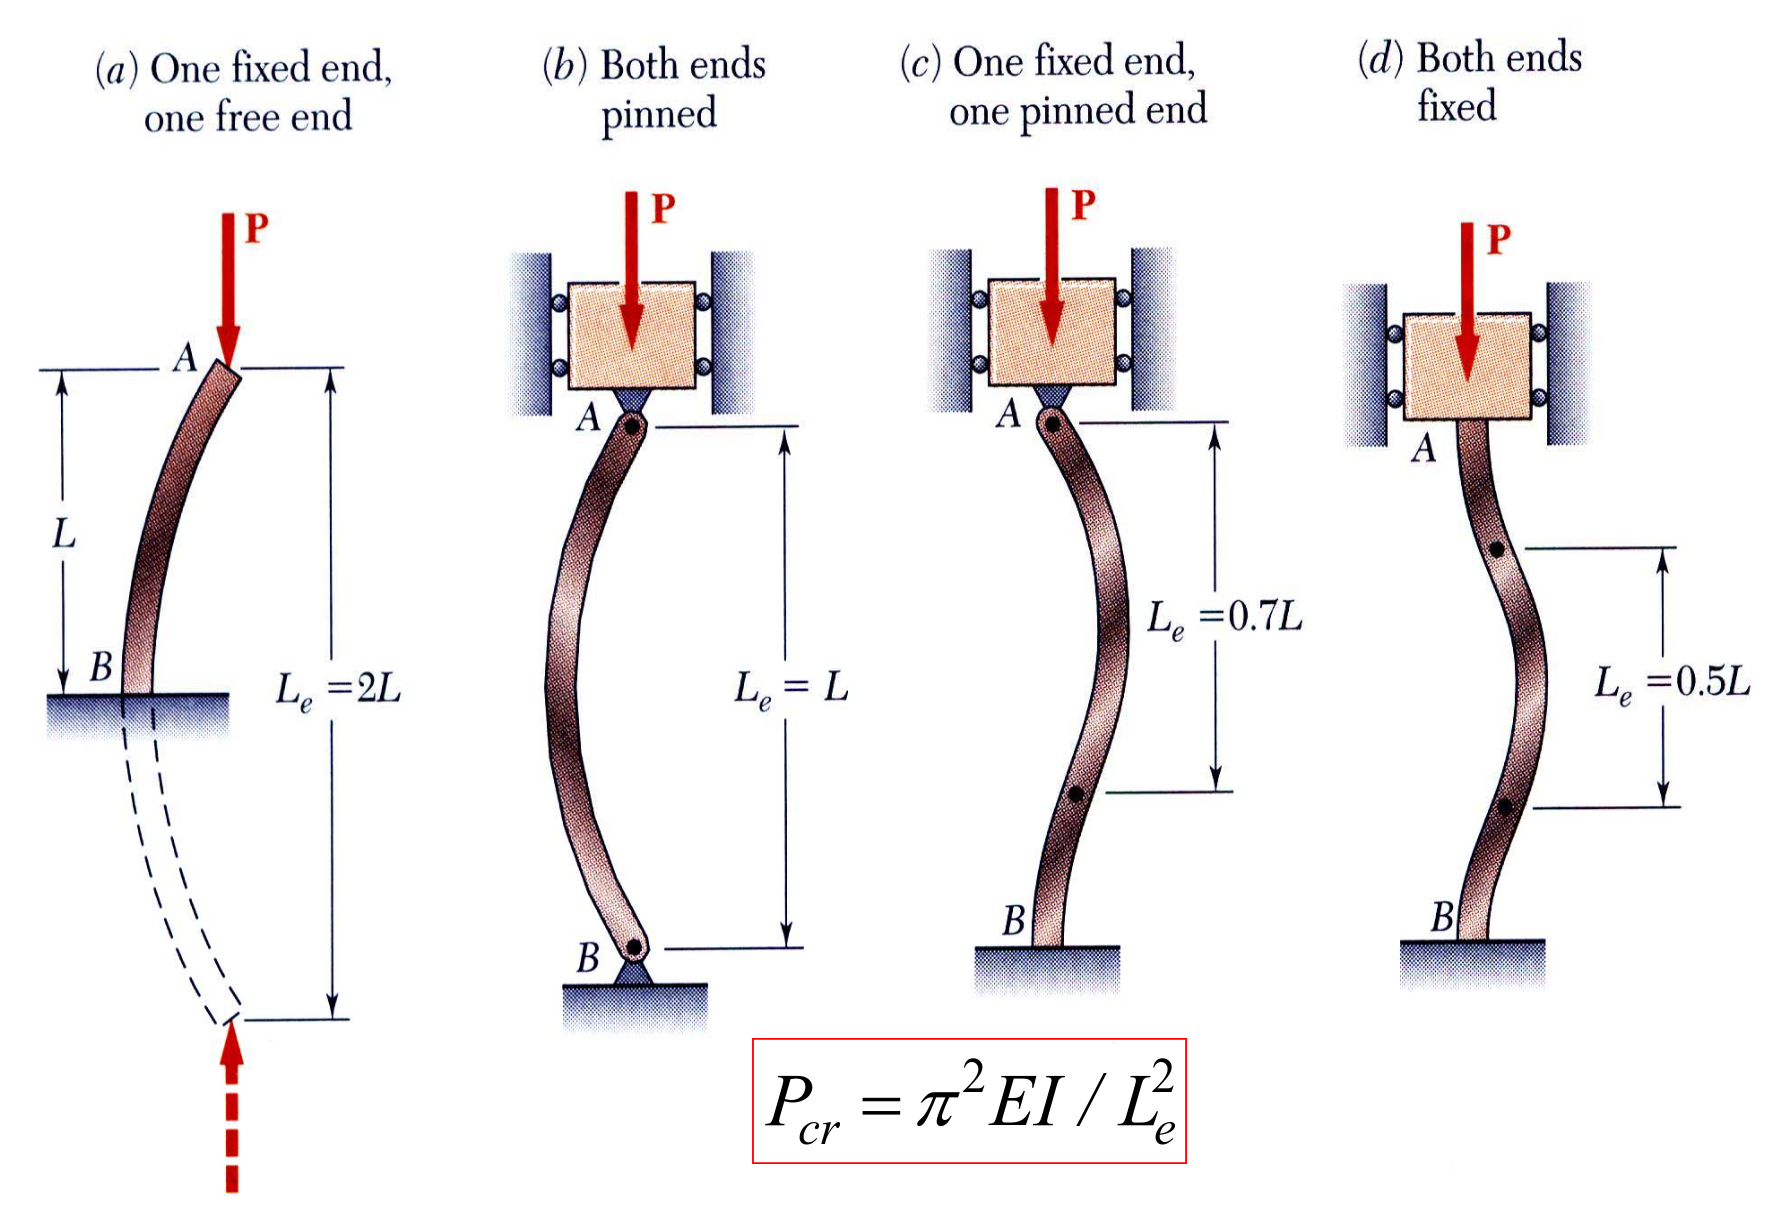
\includegraphics[width=.9\linewidth]{./images/beam-buckling.png}
\end{center}

\newpage

\section{Review of statics}
\label{sec:orgfa0b4c2}

\subsection{Tie or strut (two-force member)}
\label{sec:orge4214d7}
\begin{itemize}
\item Pin-ended members
\item Two-force member
\item Axial or longitudinal load (no bending) produces axial stresses
\item Assume that the member is weightless
\end{itemize}

\subsection{Beam}
\label{sec:org3aef0d1}
\begin{itemize}
\item Multiple internal forces
\item Pin-ended or fix-ended
\item Bending produces bending stresses and shearing stresses
\end{itemize}

\newpage

\section{Normal stress}
\label{sec:orgd906144}
\begin{itemize}
\item Stress is an \textbf{internal} force.
\item For an object in \textbf{tension}, the stress is \textbf{positive}.
\item For an object in \textbf{tension}, the cross-sectional area to calculate stress must be at the smallest area, like the hinge part of a bar.
\item For an object in \textbf{compression}, the stress is \textbf{negative}.
\item For an object in \textbf{compression}, the cross-sectional area to calculate the stress is the whole area of the bar.
\item The stress at a transition point from tension to compression or vice versa is \textbf{undefined}.
\item To figure out whether an object is in tension or compression, draw out the object and find the internal forces on the object. The internal forces must balance out the forces acting on the object. Then use the direction of the force to figure out whether the object is in compression or in tension.
\end{itemize}

\[\sigma = \frac{F}{A}\]

Where:
\begin{itemize}
\item \(\sigma\) is the normal stress
\item \(F\) is the force on the ends of the object, or the axial force on the object
\item \(A\) is the cross-sectional area
\end{itemize}


\section{Method of joints}
\label{sec:org58991ba}
\begin{itemize}
\item The object must be a two-force member, or have no transverse load on the object. Weight of the object is assumed to be negligible.
\end{itemize}


\section{Stresses in objects}
\label{sec:org73e676b}
\begin{itemize}
\item Axial forces on a two-force member result in only \textbf{normal stresses} on a plane cut perpendicular to the member axis.
\item Transverse forces on bolts and pins result in only shearing stresses on the plane perpendicular to the bolt or pins axis.
\item Either axial or transverse forces may produce both normal and shearing stresses with respect to a plane other than one cut perpendicular to the member axis.
\end{itemize}


\section{Stresses on an oblique plane}
\label{sec:org0b0456d}

\subsection{Normal stress}
\label{sec:org21cf0b6}
\[\sigma = \frac{F}{A} \cos^2 \theta\]

Where:
\begin{itemize}
\item \(\sigma\) is the normal stress
\item \(F\) is the axial force on the object
\item \(A\) is the cross-sectional are of the object
\item \(\theta\) is the angle between the normal of the oblique plane and the axial force on the object
\end{itemize}

\subsection{Shearing stress}
\label{sec:org8fe4f71}
\[\sigma = \frac{F}{A} \sin \theta \cos \theta\]

Where:
\begin{itemize}
\item \(\sigma\) is the normal stress
\item \(F\) is the axial force on the object
\item \(A\) is the cross-sectional are of the object
\item \(\theta\) is the angle between the normal of the oblique plane and the axial force on the object
\end{itemize}

\subsection{Maximum stresses}
\label{sec:orgd54a8f3}

\subsubsection{Normal stress}
\label{sec:org16974f2}
The maximum normal stress occurs when the oblique plane is perpendicular to the axis of the object.

\subsubsection{Shearing stress}
\label{sec:org12701d7}
The maximum shearing stress occurs when the oblique plane is \(\pm 45^{\circ}\) with respect to the axis of the object.


\section{Deformations under axial loading}
\label{sec:orge7c72fa}
\begin{itemize}
\item From Hooke's Law:
\[\sigma = E \varepsilon \qquad \varepsilon = \frac{\sigma}{E} = \frac{F}{AE}\]

\item From the definition of strain:
\[\varepsilon = \frac{\delta}{L} = \frac{F}{AE}\]

\item Equating and solving for the deformation:
\[\delta = \frac{FL}{AE}\]

\item With variations in loading, cross-section or material properties,
\[\delta = \sum_i \frac{F_i L_i}{A_i E_i}\]
\end{itemize}


\section{Limits (e.g. maximum shearing stress, maximum normal stress, etc.)}
\label{sec:org0684656}
The presence of limits (e.g. maximum shearing stress, maximum normal stress, etc.) usually means there is \textbf{an answer for each limit}. Each answer that is derived from a limit must then be \textbf{compared with each other} in regard to \textbf{safety} to get the final correct answer.


\section{Axial shear}
\label{sec:orgf2f9e27}
\begin{itemize}
\item Torque applied to a shaft produce \textbf{shearing stresses} on the faces perpendicular to the axis (basically the ends of a bar or a beam).
\item Equilibrium requires the existence of equal stresses on the faces of the two planes containing the axis of the shaft.
\end{itemize}


\section{Shaft deformation}
\label{sec:org8dad8ee}
\begin{itemize}
\item The twisting angle of the shaft is proportional to the applied torque and to the shaft length.

\[\phi \propto T \text{ and } \phi \propto L\]
\[\phi = \frac{TL}{GJ}\]

Where:
\begin{itemize}
\item \(\phi\) is the twisting angle of the shaft
\item \(T\) is the applied torque
\item \(L\) is the shaft length
\item \(G\) is the shear modulus
\item \(J\) is the polar moment of inertia
\end{itemize}

\item When subjected torsion, every cross-section of a circular shaft remains \textbf{planar} and undistorted.
\item Cross-sections for hollow and solid circular shafts remain planar and undistorted as a circular shaft is axisymmetric.
\item Cross-sections of non-circular (non-axisymmetric) shafts, like rectangular shafts, are distorted when subjected to torsion.
\end{itemize}


\section{Pure shear element at \(45^{\circ}\) degrees}
\label{sec:orgd257a30}
\begin{itemize}
\item There is only tension and compression, which are normal stresses.
\item There is no shearing stress on the element.
\end{itemize}

\newpage

\section{Right-hand screw rule}
\label{sec:org11d0ad2}
\begin{itemize}
\item The four fingers of your right hand must follow the direction of the torque applied.
\item The thumb will then give the torque direction.
\item The torque direction is an arrow with two arrowheads.
\end{itemize}


\section{Failure modes of a bar}
\label{sec:orgfe7ee63}

\subsection{Summary}
\label{sec:org9ff7448}
\begin{center}
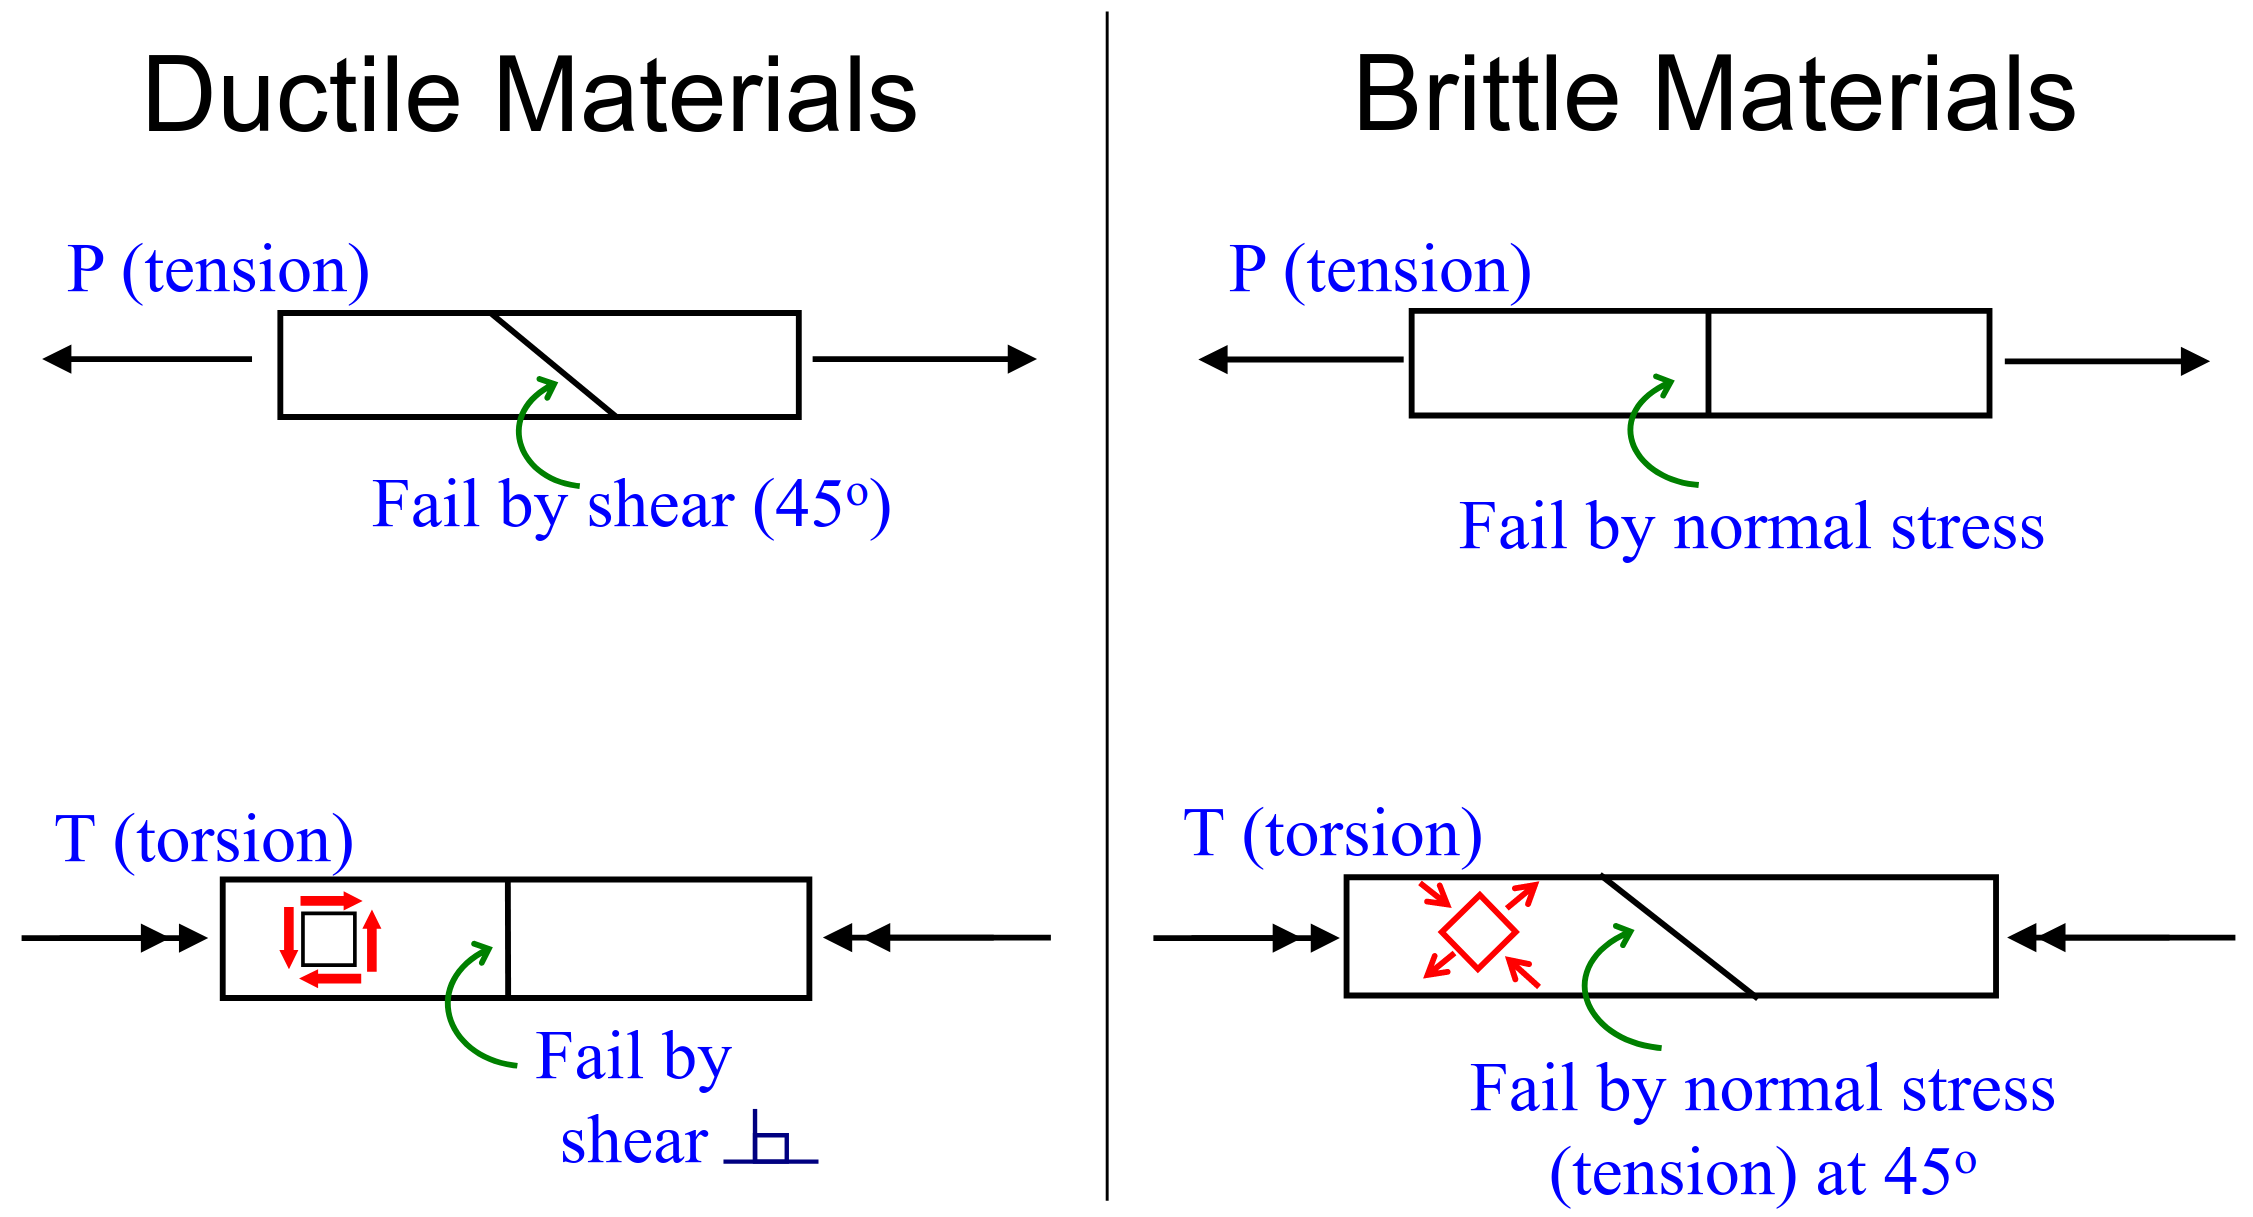
\includegraphics[width=.9\linewidth]{./images/failure-modes-summary.png}
\end{center}

\newpage

\subsection{Torsional failure modes}
\label{sec:orga49debc}

\subsubsection{Ductile materials}
\label{sec:org8201285}
\begin{itemize}
\item Ductile materials generally fail in \textbf{shear}. They are weaker in shear than in tension.
\item When subjected to torsion, a ductile material breaks along the plane of \textbf{maximum shear}, which is a plane perpendicular to the shaft's axis.
\end{itemize}

\begin{center}
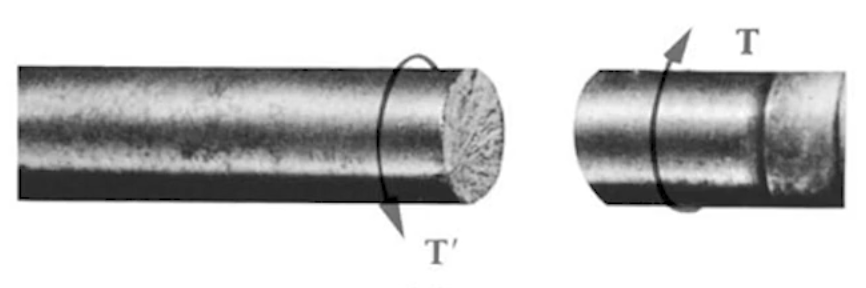
\includegraphics[width=.9\linewidth]{./images/ductile-material-torsional-failure.png}
\end{center}

\subsubsection{Brittle materials}
\label{sec:org14f01c6}
\begin{itemize}
\item Brittle materials generally fail in \textbf{tension}. They are weaker in tension than in shear.
\item When subjected to torsion, a brittle material breaks along planes perpendicular to the direction in which \textbf{tension is a maximum}, which is along surfaces at \(45^{\circ}\) to the shaft's axis.
\item This is called a spiral or helical failure.
\end{itemize}

\begin{center}
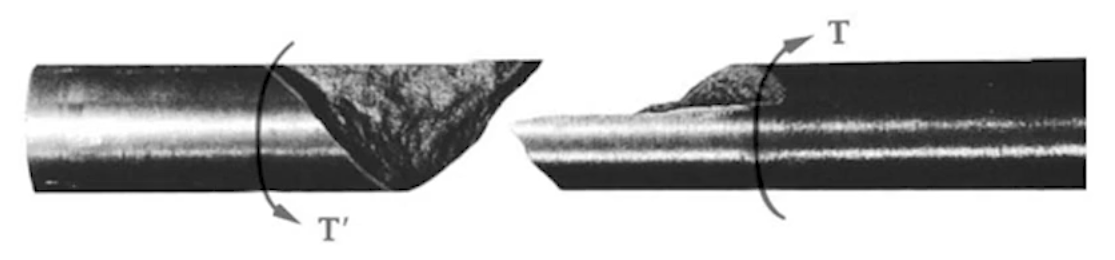
\includegraphics[width=.9\linewidth]{./images/brittle-material-torsional-failure.png}
\end{center}

\newpage

\section{Difference between torque and bending moment}
\label{sec:org5888cb1}

\subsection{Torque}
\label{sec:orgd4944e3}
Torque is the bending or twisting about the object's longitudinal axis.

\subsection{Bending moment}
\label{sec:org84e4b8b}
Bending moment is bending the object about an axis that is \textbf{perpendicular} to the member's longitudinal axis.


\section{Bending deformations}
\label{sec:orgb991b69}
For a beam with a plane of symmetry in pure bending:
\begin{itemize}
\item The beam remains symmetric.
\item The beam bends uniformly to form a circular arc.
\item The sides of the beam should pass through the centre of the circle and remain planar.
\item The length of the \textbf{top} side of the beam \textbf{decreases} and the length of the \textbf{bottom} side \textbf{increases}.
\item A neutral surface must exist that is parallel to the upper and lower surfaces and for which the length does not change.
\item Stresses and strains are \textbf{negative (compressive)} above the neutral plane or neutral surface and \textbf{positive (tensive)} below it.
\end{itemize}


\section{Finding the centroid of an irregularly-shaped object}
\label{sec:orga065442}
\[\bar{Y} = \frac{\sum \bar{y} A}{\sum A}\]

Where:
\begin{itemize}
\item \(\bar{Y}\) is the distance of the centroid from the reference plane
\item \(\bar{y}\) is the distance of the centroid of an \textbf{individual} section of the object from the reference plane
\item \(A\) is the area of each \textbf{individual} section of the object
\end{itemize}

\section{Calculating the \(I\) for an irregularly-shaped object}
\label{sec:orgcc295c6}

\subsection{Method 1: Using parallel axis theorem directly}
\label{sec:org8ee7374}
\[I = \sum \left(\bar{I} + Ad^2 \right) = \sum \left(\frac{1}{12} bh^3 + Ad^2 \right)\]

Where:
\begin{itemize}
\item \(I\) is the second moment of area of the object
\item \(\bar{I}\) is the second moment of area for an \textbf{individual} section of the object
\item \(A\) is the area of an \textbf{individual} section of the object
\item \(d\) is the distance from the centroid of the \textbf{individual} section from the centroid of the whole object
\item \(b\) is the base of an \textbf{individual} section of the object
\item \(h\) is the height of an \textbf{individual} section of the object
\end{itemize}

\newpage

\subsection{Method 2: Calculate \(I\) about the base of each rectangle}
\label{sec:org0e31e23}

\subsubsection{Finding the \(I\) about the base of the rectangle}
\label{sec:org8de8d08}
\begin{align*}
I_{base} &= I_{\text{NA}} + Ad^2 \\
&= \frac{bh^3}{12} + bh \left( \frac{h}{2} \right)^2 \\
&= \frac{bh^3}{12} + \frac{bh^3}{4} \\
&= \frac{bh^3}{3}
\end{align*}

Where:
\begin{itemize}
\item \(I_{base}\) is the second moment of area at the base of a rectangular section of the object
\item \(I_{\text{NA}}\) is the second moment of area about the neutral axis of a rectangular section of the object
\item \(b\) is the base of a rectangular section of the object
\item \(h\) is the height of a rectangular section of the object
\end{itemize}

\subsubsection{Summing up the individual \(I\)s to get the \(I\) of the object}
\label{sec:org93cd6a1}
\begin{itemize}
\item When doing this, all the rectangles taken into account must have their second moment of area (\(I\)) taken at the centroid of the object.
\item There will likely be extra space that has been considered, and hence those extra spaces that are not part of the object must be removed by subtracting from the sum below.
\item This is useful for objects that are not symmetrical about their neutral axis, such as a T shape cross-section.
\end{itemize}

\[I = \sum \left( \frac{bh^3}{3} \right)\]

Where:
\begin{itemize}
\item \(I\) is the second moment of area of the object
\item \(b\) is the base of a rectangular section of the object
\item \(h\) is the height of a rectangular section of the object
\end{itemize}

\newpage

\subsection{Method 3: Subtract smaller rectangles from a larger rectangle}
\label{sec:org8f7e73f}
\begin{itemize}
\item This method only applies when the object is symmetrical about its neutral axis, such as an I-beam.
\item The centroid of the rectangular section must \textbf{coincide} with the centroid of the object's centroid.
\end{itemize}

For an I-beam:

\begin{center}
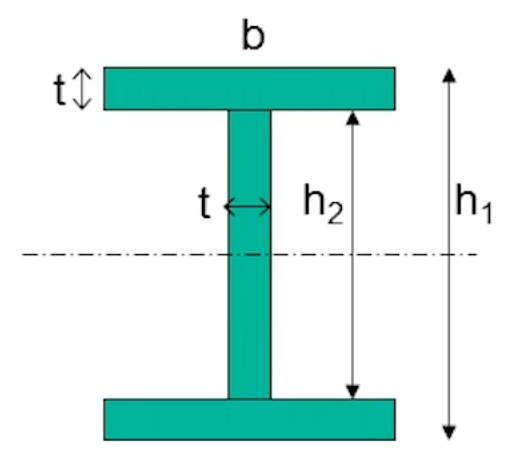
\includegraphics[scale=1]{./images/i-beam-section-moment-of-inertia.png}
\end{center}

\[I_{\text{NA}} = \frac{bh_1^3}{12} - \frac{(b - t)h_2^3}{12}\]

Where:
\begin{itemize}
\item \(I_{\text{NA}}\) is the second moment of area of the I-beam
\item \(b\) is the base of the I-beam
\item \(h_1\) is the height of the I-beam
\item \(t\) is the width of the middle section of the I-beam
\item \(h_2\) is the distance between the bottom part of the I-beam and the top part of the I-beam
\end{itemize}


\section{Eccentric Axial Loading}
\label{sec:org468b371}

\subsection{Determining the resultant force and bending moment on the centroid}
\label{sec:orgaeb3f7a}
\begin{enumerate}
\item Transfer the applied force to the centroid of the section and use that applied force to calculate the moment about the centroid
\item Determine the force and the moment using equilibrium equations. Assume a direction for the force and the moment and equate the resultant to zero to find the actual magnitude and direction of the force and the moment.
\end{enumerate}

\subsection{General case of eccentric axial loading}
\label{sec:org6853d5e}
\begin{itemize}
\item Consider a straight member subject to equal and opposite eccentric forces.
\item The eccentric force is equivalent to the system of a centric force and two bending moments.
\item The stress at any point can be obtained using the principle of superposition.
\item The sign of the stress can be determined through visualisation.
\end{itemize}

\newpage

\section{Types of supports and their corresponding forces}
\label{sec:orgecdca68}
\begin{center}
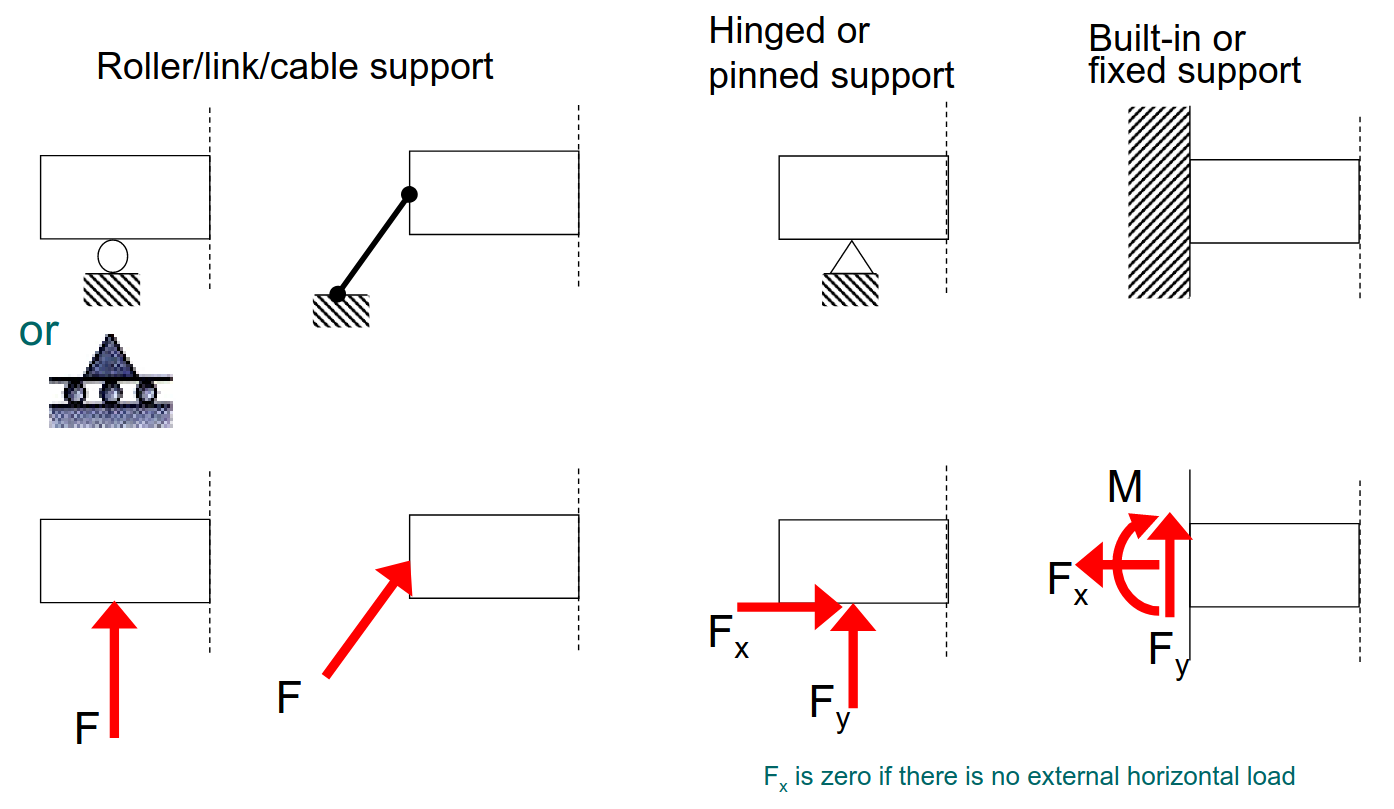
\includegraphics[width=.9\linewidth]{./images/types-of-supports.png}
\end{center}

\section{Beam types}
\label{sec:org67ed69c}

\subsection{Statically determinate beams}
\label{sec:org3124273}

\subsubsection{Simply supported beams}
\label{sec:orga91899d}
Simply supported beams have a fixed end on the left and a roller on the right end.
\begin{center}
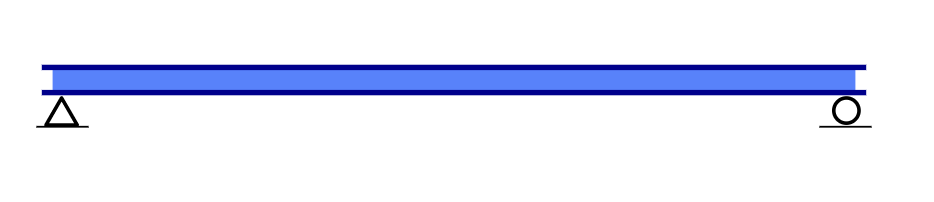
\includegraphics[width=.9\linewidth]{./images/simply-supported-beam-type.png}
\end{center}

\subsubsection{Cantilever beams}
\label{sec:orgacf5286}
Cantilever beams are supported from one end, with a fixed support.
\begin{center}
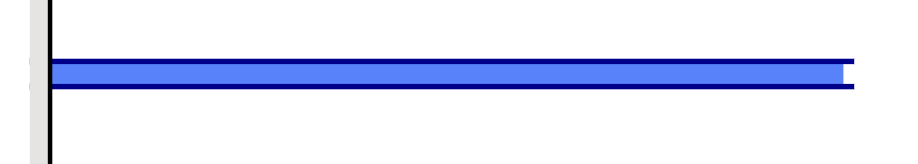
\includegraphics[width=.9\linewidth]{./images/cantilever-beam-type.png}
\end{center}

\subsection{Statically indeterminate beams}
\label{sec:org0e3eedb}

\subsubsection{Continuous beams}
\label{sec:orgc4789bf}
Continuous beams are multi-spanned beams with multiple supports across the length of the beam.
\begin{center}
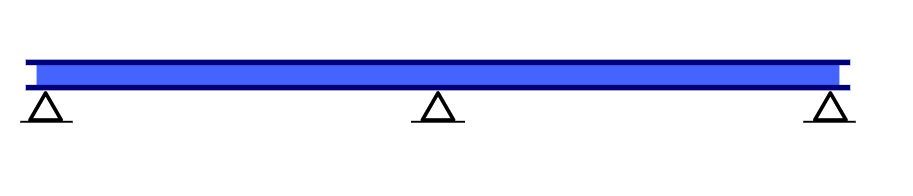
\includegraphics[width=.9\linewidth]{./images/continuous-beam-type.png}
\end{center}

\subsubsection{Fixed beams}
\label{sec:orgd6e6e4b}
Fixed beams have fixed supports on either end.
\begin{center}
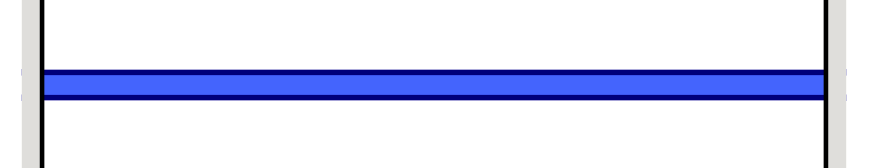
\includegraphics[width=.9\linewidth]{./images/fixed-beam-type.png}
\end{center}

\subsubsection{Overhanging beams}
\label{sec:org0d8bd9b}
Overhanging beams are beams with two supports, but one of the supports is not at the end of the beam.
\begin{center}
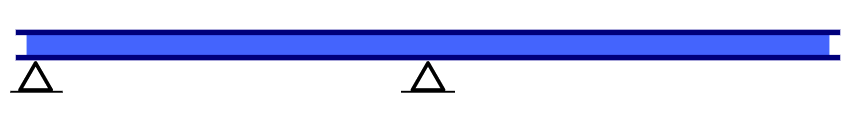
\includegraphics[width=.9\linewidth]{./images/overhanging-beam-type.png}
\end{center}

\newpage

\section{Sign conventions}
\label{sec:org54cc58a}
\begin{enumerate}
\item \textbf{Smiley face} or sagging action is considered \textbf{positive bending moment}.
\begin{center}
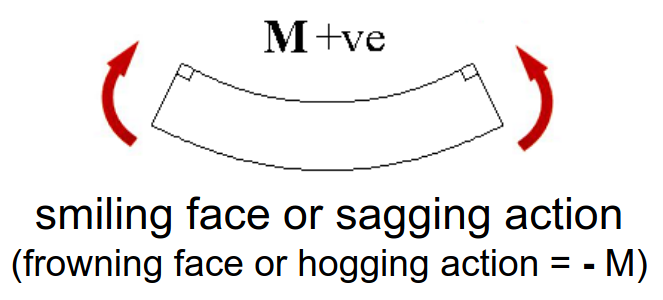
\includegraphics[scale=0.6]{./images/bending-moment-sign-convention.png}
\end{center}

\item A \textbf{clockwise rotation} is considered positive shear \textbf{force}.
\begin{center}
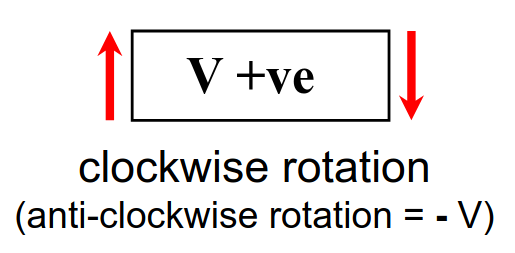
\includegraphics[scale=0.6]{./images/shear-force-sign-convention.png}
\end{center}

\item \textbf{Tension} is \textbf{positive} normal stress.
\begin{center}
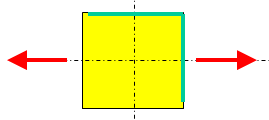
\includegraphics[scale=0.5]{./images/positive-normal-stress.png}
\end{center}

\item \textbf{Shearing stress} is considered \textbf{positive} when the \textbf{right-hand side} of the element has an arrow pointing \textbf{upwards}. Another way to think of it is that the line formed by the arrows of the shearing stress is \textbf{positive} when the line has a \textbf{positive gradient}.
\begin{center}
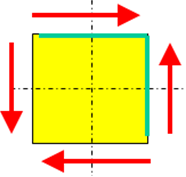
\includegraphics[scale=0.7]{./images/positive-shear-stress.png}
\end{center}

\item \textbf{Internal forces} should always be assumed to be \textbf{positive}.
\item The moment at unconstrained ends must be 0.
\end{enumerate}

\newpage

\subsubsection{Applying the sign conventions}
\label{sec:orgfc5f951}
\begin{itemize}
\item These sign conventions only apply when the beam is cut on the right side of the beam, which means the cut part has the \textbf{fixed end on the right} and the \textbf{free end on the left}.
\item If the beam is cut on the left side of the beam, which means the cut part has the \textbf{fixed end on the left} and the \textbf{free end on the right}, the sign conventions are \textbf{reversed}.
\end{itemize}

\section{Bending moment and shear force diagrams}
\label{sec:orgb224ec0}

\subsection{Free body diagram method}
\label{sec:org2b2d1fc}
\begin{enumerate}
\item Draw free body diagrams for each section of interest.
\item Start drawing the free body diagrams starting from both sides so that the answer can be checked.
\item If the final result in the middle calculated both sides are the same, then the answer is most probably correct.
\item Assume internal forces to be positive, which means the bending moment forms a smiley face and the shear force causes a clockwise rotation.
\item Use the equilibrium expressions \(\sum M_i = 0\) and \(\sum F_i = 0\) to find the internal forces.
\item Alternatively, the sign conventions above can also be used to find the internal forces.
\item Distributed loads must always be assumed to act at the centre of the segment of interest after obtaining the total load.
\end{enumerate}

\newpage

\subsection{Direct method for shear force diagrams}
\label{sec:org3a047e0}
\begin{enumerate}
\item Start from the left of the beam and move across the beam.
\item The shear force starts from zero.
\item When a point load is encountered, add the shear force due to it to the current shear force value. Use the sign convention of upwards shear forces being positive and downwards shear forces being negative. The shear force diagram should have a vertical line to the new shear force value.
\item When a distributed load is encountered, find the effective increase or decrease in shear force due to the distributed load by treating it as a point load. Then, draw a straight line to the new value of the shear force at the end of the distributed load region.
\item Alternatively, jumping over to the right side of the beam and doing point 3 in reverse will also work. Essentially, when working from the right side of the beam, the sign conventions are flipped, so a shear force acting downwards will be considered as positive while a shear force acting upwards will be considered negative and so on.
\end{enumerate}

\subsection{Relationship between load and shear force}
\label{sec:org0a60112}
\begin{align*}
\sum F_y &= 0 \\
V &= (V + \Delta V) + w \Delta x \\
\Delta V &= -w \Delta x \tag{1}
\end{align*}

Dividing both sides of \((1)\) by \(\Delta x\) and let \(\Delta x \rightarrow 0\):
\[\frac{dV}{dx} = -w\]

Where:
\begin{itemize}
\item \(\sum F_y\) is the sum of the forces in the y-axis on a segment of the object
\item \(V\) is the shear force on a segment of the object
\item \(\Delta V\) is the change in the shear force due to the distributed load
\item \(w\) is the distributed load on a segment of the object
\item \(\Delta x\) is the length of a segment of the object
\item \(\frac{dV}{dx}\) is the change in shear force over the length of the object
\end{itemize}

\subsubsection{Implications}
\label{sec:org720d7be}
\begin{itemize}
\item When there is \textbf{no} distributed load, i.e. \(w = 0\), the shear force is \textbf{constant}.
\item When there is a \textbf{distributed} load, i.e. \(w \ne 0\), the shear force has a \textbf{linear} variation.
\item The net change in bending moment is equal to the area under the shear distribution segments, i.e:
\[\text{Change in bending moment, } \Delta M = \text{Area under the shear force diagram}\]
\end{itemize}

\subsection{Relationship between shear force and bending moment}
\label{sec:org0daafce}
\begin{align*}
\sum M &= 0 \\
(M + \Delta M) + w \Delta x \left(\frac{\Delta x}{2} \right) &= M + V \Delta x \\
\Delta M &= V \Delta x - \frac{1}{2}w\left(\Delta x \right)^2 \\
\Delta M &= (V - \frac{1}{2} w \Delta x) \Delta x \tag{2}
\end{align*}

Dividing both sides of \((2)\) by \(\Delta x\) and let \(\Delta x \rightarrow 0\):
\[\frac{dM}{dx} = V\]

Where:
\begin{itemize}
\item \(\sum M\) is the sum of moments about a pivot in a segment of the object
\item \(M\) is the bending moment on a segment of the object
\item \(\Delta M\) is the change in the bending moment due to the distributed load
\item \(w\) is the distributed load on a segment of the object
\item \(\Delta x\) is the length of a segment of the object
\item \(V\) is the shear force on a segment of the object
\item \(\frac{dM}{dx}\) is the change in bending moment over the length of the object
\end{itemize}

\subsubsection{Implications}
\label{sec:orgda04e9a}
\begin{itemize}
\item The variation in bending moment is \textbf{linear} when the shear force is \textbf{constant}, i.e. \(\frac{dV}{dx} = 0\).
\item The variation in bending moment is \textbf{quadratic} when the shear force is \textbf{not} constant, i.e. \(\frac{dV}{dx} \ne 0\).
\item The bending moment is \textbf{maximum or minimum} when the shear force is zero, or when the shear force line crosses the zero line. Basically, there is a \textbf{turning point} in the bending moment diagram whenever the \textbf{shear force is zero}.
\item The bending moment at \textbf{free ends} must be \textbf{zero}.
\end{itemize}

\newpage

\section{Design of beams for bending}
\label{sec:org0cc8846}
\begin{itemize}
\item The largest normal stress is found at the \textbf{surface} where the maximum bending moment occurs.
\[\sigma_m = \frac{|M|_{max} c}{L} = \frac{|M|_{max}}{S}\]

Where:
\begin{itemize}
\item \(\sigma_m\) is the maximum normal stress
\item \(|M|_{max}\) is the absolute value of the maximum bending moment
\item \(c\) is the outer radius of the beam
\item \(L\) is the length of the beam
\item \(S\) is the section modulus of the beam
\end{itemize}

\item A safe design requires that the maximum normal stress be lower that the allowable stress for the material used. These criteria lead to the determination of the minimum acceptable section modulus.
\[\sigma_m \le \sigma_{all}\]
\[\sigma_{all} = \frac{|M|_{max}}{S_{min}}\]
\[S_{min} = \frac{|M|_{max}}{\sigma_{all}}\]

Where:
\begin{itemize}
\item \(\sigma_m\) is the maximum normal stress
\item \(\sigma_{all}\) is the allowable normal stress
\item \(|M|_{max}\) is the absolute value of the maximum bending moment
\item \(S_{min}\) is the minimum section modulus of the beam
\end{itemize}
\end{itemize}

\newpage

\section{Yield criteria}
\label{sec:org4b20ef8}

\subsection{Ductile materials}
\label{sec:org1c17777}
\begin{itemize}
\item Mild steel (steel with low amounts of carbon)
\item Aluminium alloy
\end{itemize}

\subsubsection{Maximum shearing stress criteria (Tresca) criterion}
\label{sec:org0c2c1f3}
Use the \textbf{maximum out-of-plane} shearing stress if it exists.
\[\tau_{max} < \frac{\sigma_Y}{2}\]

Where:
\begin{itemize}
\item \(\sigma_Y\) is the material yield stress
\item \(\tau_{max}\) is the maximum shearing stress
\end{itemize}

\subsubsection{Maximum distortion energy (Von Mises) criterion}
\label{sec:orgdc6528b}
\[\sigma_{max}^2 - \sigma_{max} \sigma_{min} + \sigma_{min}^2 < \sigma_Y^2\]

Where:
\begin{itemize}
\item \(\sigma_{max}\) is the maximum normal stress
\item \(\sigma_{min}\) is the minimum normal stress
\item \(\sigma_{Y}\) is the material yield stress
\end{itemize}

\newpage

\subsection{Brittle materials}
\label{sec:orgce901b6}
\begin{itemize}
\item Brittle materials fail suddenly through rupture or fracture.
\item Failure condition is characterised by \textbf{ultimate strength \(\boldsymbol{\sigma_U}\)}.
\end{itemize}

Examples:
\begin{itemize}
\item Cast iron
\item Glass
\item Ceramics
\end{itemize}

\subsubsection{Maximum normal stress (Coulomb's) criterion}
\label{sec:org3412e1e}
\[|\sigma_{max}| < \sigma_U\]
\[|\sigma_{min}| < \sigma_U\]

Where:
\begin{itemize}
\item \(\sigma_{max}\) is the maximum normal stress
\item \(\sigma_{min}\) is the minimum normal stress
\item \(\sigma_U\) is the ultimate strength of the material
\end{itemize}

\subsection{Factor of safety consideration}
\label{sec:org5aaf42d}
When a factor of safety needs to be taken into account, divide the stress used in the criterion by the factor of safety.

\subsubsection{Maximum shearing stress criteria (Tresca) criterion}
\label{sec:org863bffc}
Use the \textbf{maximum out-of-plane} shearing stress if it exists.
\[\tau_{max} < \frac{\sigma_Y}{2FS}\]

Where:
\begin{itemize}
\item \(\sigma_Y\) is the material yield stress
\item \(\tau_{max}\) is the maximum shearing stress
\item \(FS\) is the factor of safety
\end{itemize}

\subsubsection{Maximum distortion energy (Von Mises) criterion}
\label{sec:org22c9d7e}
\[\sigma_{max}^2 - \sigma_{max} \sigma_{min} + \sigma_{min}^2 < \left(\frac{\sigma_Y}{FS} \right)^2\]

Where:
\begin{itemize}
\item \(\sigma_{max}\) is the maximum normal stress
\item \(\sigma_{min}\) is the minimum normal stress
\item \(\sigma_{Y}\) is the material yield stress
\item \(FS\) is the factor of safety
\end{itemize}

\subsubsection{Maximum normal stress (Coulomb's) criterion}
\label{sec:org74b0cdb}
\[|\sigma_{max}| < \frac{\sigma_U}{FS}\]
\[|\sigma_{min}| < \frac{\sigma_U}{FS}\]

Where:
\begin{itemize}
\item \(\sigma_{max}\) is the maximum normal stress
\item \(\sigma_{min}\) is the minimum normal stress
\item \(\sigma_U\) is the ultimate strength of the material
\item \(FS\) is the factor of safety
\end{itemize}

\newpage

\section{Deflection of beams}
\label{sec:org6235329}
Use the elastic curve and singularity function to find the deflection of beams.
\begin{itemize}
\item Assume small deflection \(\theta < \qty{5.73}{\degree}\).
\item Begin with the origin on the left end of the beam and cut last section on the right.
\item For distributed loads, extend to the distributed load all the way until the right end of the beam and cancel the excess distributed load with another distributed load.
\item Use symmetry of the beam if possible, but take note that the boundary condition at the point of symmetry is \(\boldsymbol{y' = 0}\).
\end{itemize}

\subsection{Elastic curve equation}
\label{sec:org01bbff8}
\[EIy'' = M(x)\]
\[EIy' = \int_0^x M(x) \, dx + C_1\]
\[EIy = \int_0^x \, dx \int_0^x M(x) \, dx + C_1 x + C_2\]

Where:
\begin{itemize}
\item \(E\) is the modulus of elasticity
\item \(I\) is the second moment of area
\item \(M\) is the bending moment of the beam, expressed as a function of \(x\), or the distance from the left end of the beam
\item \(y\) is the general equation for the deflection of the beam at any point. It is a function of \(x\) or the distance from the left end of the beam.
\end{itemize}

\newpage

\subsection{Singularity function method}
\label{sec:orge61f9f4}

\subsubsection{Rules}
\label{sec:org301f83d}
\begin{itemize}
\item The distance \(x\) must be within the last section of the beam, which is on the right of the origin.
\item You \textbf{cannot expand} a singularity function (<\ldots{}>).
\item When finding constants using boundary conditions, \textbf{ignore} the content inside the singularity function (<\ldots{}>) if it is \textbf{negative}.
\item If the content inside the singularity function (<\ldots{}>) is \textbf{positive}, \textbf{include} it.
\item Find constants \(C_1\) and \(C_2\) using boundary conditions of zero or known deflection or slope.
\begin{itemize}
\item For pinned ends, \(y = 0\) when \(x = 0\) and \(x = L\).
\item For clamped ends, \(y = 0\) and \(y' = 0\) when \(x = 0\) and \(x = L\).
\end{itemize}
\end{itemize}

\subsubsection{Distributed load}
\label{sec:orgb33c6a5}
\[\frac{w}{2} < x - x_0 >^2\]

Where:
\begin{itemize}
\item \(w\) is the distributed load
\item \(x\) is a \textbf{variable} representing the distance from the \textbf{left end} of the beam
\item \(x_0\) is the location of the \textbf{left end} of the distributed load measured from the \textbf{left end} of the beam.
\end{itemize}

\subsubsection{Point load}
\label{sec:orgc69cce9}
\[F_p < x - x_0 >\]

Where:
\begin{itemize}
\item \(F_p\) is the point load
\item \(x\) is a \textbf{variable} representing the distance from the \textbf{left end} of the beam
\item \(x_0\) is the location of the point load measured from the \textbf{left end} of the beam
\end{itemize}

\subsubsection{Point moments}
\label{sec:orgadab504}
\[M < x - x_0 >^0\]

Where:
\begin{itemize}
\item \(M\) is the point moment
\item \(x\) is a \textbf{variable} representing the distance from the \textbf{left end} of the beam
\item \(x_0\) is the location of the point moment measured from the \textbf{left end} of the beam
\end{itemize}

\subsection{Figuring out the point of maximum deflection}
\label{sec:orgf113768}
\begin{itemize}
\item For a single point load in the middle of the beam, the point of maximum deflection will be at the middle of the beam.
\item When the point load is moved to one side of a beam, the point of maximum deflection will move with the point load, but it'll lag behind.
\item This means that the point of maximum deflection will be closer to the middle of the beam compared to the position of the point load when the point load is not at the middle of the beam.
\end{itemize}

\newpage

\section{Important points to note}
\label{sec:orgecc617e}
\begin{enumerate}
\item Forces on an object is assumed to act on the \textbf{centroid} unless otherwise stated.
\item Stresses on a point or an element is assumed to be on the \textbf{surface} of the structure.
\item The word \textbf{'force'} means a force-type quantity, including a concentrated force (\(\unit{N}\)), moment (\(\unit{N.m}\)), or a torque (\(\unit{N.m}\))
\item Internal forces on a member can be \textbf{action} or \textbf{reaction (equilibrium)} forces.
\item Offset loads must be transferred to the \textbf{centroid} at the cross-section of interest.
\item \textbf{Action} forces or \textbf{reaction (equilibrium)} forces must result in the same stresses on a particular element.
\item Sign conventions are \textbf{reversed} when cutting the left side of the beam. Usually, the cuts are on the right side of the beam, not the left.
\end{enumerate}
\end{document}
